% Options for packages loaded elsewhere
\PassOptionsToPackage{unicode}{hyperref}
\PassOptionsToPackage{hyphens}{url}
\PassOptionsToPackage{dvipsnames,svgnames,x11names}{xcolor}
%
\documentclass[
  letterpaper,
  DIV=11,
  numbers=noendperiod]{scrartcl}

\usepackage{amsmath,amssymb}
\usepackage{iftex}
\ifPDFTeX
  \usepackage[T1]{fontenc}
  \usepackage[utf8]{inputenc}
  \usepackage{textcomp} % provide euro and other symbols
\else % if luatex or xetex
  \usepackage{unicode-math}
  \defaultfontfeatures{Scale=MatchLowercase}
  \defaultfontfeatures[\rmfamily]{Ligatures=TeX,Scale=1}
\fi
\usepackage{lmodern}
\ifPDFTeX\else  
    % xetex/luatex font selection
\fi
% Use upquote if available, for straight quotes in verbatim environments
\IfFileExists{upquote.sty}{\usepackage{upquote}}{}
\IfFileExists{microtype.sty}{% use microtype if available
  \usepackage[]{microtype}
  \UseMicrotypeSet[protrusion]{basicmath} % disable protrusion for tt fonts
}{}
\makeatletter
\@ifundefined{KOMAClassName}{% if non-KOMA class
  \IfFileExists{parskip.sty}{%
    \usepackage{parskip}
  }{% else
    \setlength{\parindent}{0pt}
    \setlength{\parskip}{6pt plus 2pt minus 1pt}}
}{% if KOMA class
  \KOMAoptions{parskip=half}}
\makeatother
\usepackage{xcolor}
\setlength{\emergencystretch}{3em} % prevent overfull lines
\setcounter{secnumdepth}{-\maxdimen} % remove section numbering
% Make \paragraph and \subparagraph free-standing
\makeatletter
\ifx\paragraph\undefined\else
  \let\oldparagraph\paragraph
  \renewcommand{\paragraph}{
    \@ifstar
      \xxxParagraphStar
      \xxxParagraphNoStar
  }
  \newcommand{\xxxParagraphStar}[1]{\oldparagraph*{#1}\mbox{}}
  \newcommand{\xxxParagraphNoStar}[1]{\oldparagraph{#1}\mbox{}}
\fi
\ifx\subparagraph\undefined\else
  \let\oldsubparagraph\subparagraph
  \renewcommand{\subparagraph}{
    \@ifstar
      \xxxSubParagraphStar
      \xxxSubParagraphNoStar
  }
  \newcommand{\xxxSubParagraphStar}[1]{\oldsubparagraph*{#1}\mbox{}}
  \newcommand{\xxxSubParagraphNoStar}[1]{\oldsubparagraph{#1}\mbox{}}
\fi
\makeatother

\usepackage{color}
\usepackage{fancyvrb}
\newcommand{\VerbBar}{|}
\newcommand{\VERB}{\Verb[commandchars=\\\{\}]}
\DefineVerbatimEnvironment{Highlighting}{Verbatim}{commandchars=\\\{\}}
% Add ',fontsize=\small' for more characters per line
\usepackage{framed}
\definecolor{shadecolor}{RGB}{241,243,245}
\newenvironment{Shaded}{\begin{snugshade}}{\end{snugshade}}
\newcommand{\AlertTok}[1]{\textcolor[rgb]{0.68,0.00,0.00}{#1}}
\newcommand{\AnnotationTok}[1]{\textcolor[rgb]{0.37,0.37,0.37}{#1}}
\newcommand{\AttributeTok}[1]{\textcolor[rgb]{0.40,0.45,0.13}{#1}}
\newcommand{\BaseNTok}[1]{\textcolor[rgb]{0.68,0.00,0.00}{#1}}
\newcommand{\BuiltInTok}[1]{\textcolor[rgb]{0.00,0.23,0.31}{#1}}
\newcommand{\CharTok}[1]{\textcolor[rgb]{0.13,0.47,0.30}{#1}}
\newcommand{\CommentTok}[1]{\textcolor[rgb]{0.37,0.37,0.37}{#1}}
\newcommand{\CommentVarTok}[1]{\textcolor[rgb]{0.37,0.37,0.37}{\textit{#1}}}
\newcommand{\ConstantTok}[1]{\textcolor[rgb]{0.56,0.35,0.01}{#1}}
\newcommand{\ControlFlowTok}[1]{\textcolor[rgb]{0.00,0.23,0.31}{\textbf{#1}}}
\newcommand{\DataTypeTok}[1]{\textcolor[rgb]{0.68,0.00,0.00}{#1}}
\newcommand{\DecValTok}[1]{\textcolor[rgb]{0.68,0.00,0.00}{#1}}
\newcommand{\DocumentationTok}[1]{\textcolor[rgb]{0.37,0.37,0.37}{\textit{#1}}}
\newcommand{\ErrorTok}[1]{\textcolor[rgb]{0.68,0.00,0.00}{#1}}
\newcommand{\ExtensionTok}[1]{\textcolor[rgb]{0.00,0.23,0.31}{#1}}
\newcommand{\FloatTok}[1]{\textcolor[rgb]{0.68,0.00,0.00}{#1}}
\newcommand{\FunctionTok}[1]{\textcolor[rgb]{0.28,0.35,0.67}{#1}}
\newcommand{\ImportTok}[1]{\textcolor[rgb]{0.00,0.46,0.62}{#1}}
\newcommand{\InformationTok}[1]{\textcolor[rgb]{0.37,0.37,0.37}{#1}}
\newcommand{\KeywordTok}[1]{\textcolor[rgb]{0.00,0.23,0.31}{\textbf{#1}}}
\newcommand{\NormalTok}[1]{\textcolor[rgb]{0.00,0.23,0.31}{#1}}
\newcommand{\OperatorTok}[1]{\textcolor[rgb]{0.37,0.37,0.37}{#1}}
\newcommand{\OtherTok}[1]{\textcolor[rgb]{0.00,0.23,0.31}{#1}}
\newcommand{\PreprocessorTok}[1]{\textcolor[rgb]{0.68,0.00,0.00}{#1}}
\newcommand{\RegionMarkerTok}[1]{\textcolor[rgb]{0.00,0.23,0.31}{#1}}
\newcommand{\SpecialCharTok}[1]{\textcolor[rgb]{0.37,0.37,0.37}{#1}}
\newcommand{\SpecialStringTok}[1]{\textcolor[rgb]{0.13,0.47,0.30}{#1}}
\newcommand{\StringTok}[1]{\textcolor[rgb]{0.13,0.47,0.30}{#1}}
\newcommand{\VariableTok}[1]{\textcolor[rgb]{0.07,0.07,0.07}{#1}}
\newcommand{\VerbatimStringTok}[1]{\textcolor[rgb]{0.13,0.47,0.30}{#1}}
\newcommand{\WarningTok}[1]{\textcolor[rgb]{0.37,0.37,0.37}{\textit{#1}}}

\providecommand{\tightlist}{%
  \setlength{\itemsep}{0pt}\setlength{\parskip}{0pt}}\usepackage{longtable,booktabs,array}
\usepackage{calc} % for calculating minipage widths
% Correct order of tables after \paragraph or \subparagraph
\usepackage{etoolbox}
\makeatletter
\patchcmd\longtable{\par}{\if@noskipsec\mbox{}\fi\par}{}{}
\makeatother
% Allow footnotes in longtable head/foot
\IfFileExists{footnotehyper.sty}{\usepackage{footnotehyper}}{\usepackage{footnote}}
\makesavenoteenv{longtable}
\usepackage{graphicx}
\makeatletter
\def\maxwidth{\ifdim\Gin@nat@width>\linewidth\linewidth\else\Gin@nat@width\fi}
\def\maxheight{\ifdim\Gin@nat@height>\textheight\textheight\else\Gin@nat@height\fi}
\makeatother
% Scale images if necessary, so that they will not overflow the page
% margins by default, and it is still possible to overwrite the defaults
% using explicit options in \includegraphics[width, height, ...]{}
\setkeys{Gin}{width=\maxwidth,height=\maxheight,keepaspectratio}
% Set default figure placement to htbp
\makeatletter
\def\fps@figure{htbp}
\makeatother
% definitions for citeproc citations
\NewDocumentCommand\citeproctext{}{}
\NewDocumentCommand\citeproc{mm}{%
  \begingroup\def\citeproctext{#2}\cite{#1}\endgroup}
\makeatletter
 % allow citations to break across lines
 \let\@cite@ofmt\@firstofone
 % avoid brackets around text for \cite:
 \def\@biblabel#1{}
 \def\@cite#1#2{{#1\if@tempswa , #2\fi}}
\makeatother
\newlength{\cslhangindent}
\setlength{\cslhangindent}{1.5em}
\newlength{\csllabelwidth}
\setlength{\csllabelwidth}{3em}
\newenvironment{CSLReferences}[2] % #1 hanging-indent, #2 entry-spacing
 {\begin{list}{}{%
  \setlength{\itemindent}{0pt}
  \setlength{\leftmargin}{0pt}
  \setlength{\parsep}{0pt}
  % turn on hanging indent if param 1 is 1
  \ifodd #1
   \setlength{\leftmargin}{\cslhangindent}
   \setlength{\itemindent}{-1\cslhangindent}
  \fi
  % set entry spacing
  \setlength{\itemsep}{#2\baselineskip}}}
 {\end{list}}
\usepackage{calc}
\newcommand{\CSLBlock}[1]{\hfill\break\parbox[t]{\linewidth}{\strut\ignorespaces#1\strut}}
\newcommand{\CSLLeftMargin}[1]{\parbox[t]{\csllabelwidth}{\strut#1\strut}}
\newcommand{\CSLRightInline}[1]{\parbox[t]{\linewidth - \csllabelwidth}{\strut#1\strut}}
\newcommand{\CSLIndent}[1]{\hspace{\cslhangindent}#1}

\KOMAoption{captions}{tableheading}
\makeatletter
\@ifpackageloaded{caption}{}{\usepackage{caption}}
\AtBeginDocument{%
\ifdefined\contentsname
  \renewcommand*\contentsname{Table of contents}
\else
  \newcommand\contentsname{Table of contents}
\fi
\ifdefined\listfigurename
  \renewcommand*\listfigurename{List of Figures}
\else
  \newcommand\listfigurename{List of Figures}
\fi
\ifdefined\listtablename
  \renewcommand*\listtablename{List of Tables}
\else
  \newcommand\listtablename{List of Tables}
\fi
\ifdefined\figurename
  \renewcommand*\figurename{Figure}
\else
  \newcommand\figurename{Figure}
\fi
\ifdefined\tablename
  \renewcommand*\tablename{Table}
\else
  \newcommand\tablename{Table}
\fi
}
\@ifpackageloaded{float}{}{\usepackage{float}}
\floatstyle{ruled}
\@ifundefined{c@chapter}{\newfloat{codelisting}{h}{lop}}{\newfloat{codelisting}{h}{lop}[chapter]}
\floatname{codelisting}{Listing}
\newcommand*\listoflistings{\listof{codelisting}{List of Listings}}
\makeatother
\makeatletter
\makeatother
\makeatletter
\@ifpackageloaded{caption}{}{\usepackage{caption}}
\@ifpackageloaded{subcaption}{}{\usepackage{subcaption}}
\makeatother
<script async src="https://pagead2.googlesyndication.com/pagead/js/adsbygoogle.js?client=ca-pub-1440105407870599" crossorigin="anonymous"></script>

\ifLuaTeX
  \usepackage{selnolig}  % disable illegal ligatures
\fi
\usepackage{bookmark}

\IfFileExists{xurl.sty}{\usepackage{xurl}}{} % add URL line breaks if available
\urlstyle{same} % disable monospaced font for URLs
\hypersetup{
  pdftitle={Chương 1: Đại cương về kỹ thuật chiết xuất},
  pdfauthor={TS. Hoàng Lê Sơn},
  colorlinks=true,
  linkcolor={blue},
  filecolor={Maroon},
  citecolor={Blue},
  urlcolor={Blue},
  pdfcreator={LaTeX via pandoc}}


\title{Chương 1: Đại cương về kỹ thuật chiết xuất}
\author{TS. Hoàng Lê Sơn}
\date{}

\begin{document}
\maketitle

\renewcommand*\contentsname{Table of contents}
{
\hypersetup{linkcolor=}
\setcounter{tocdepth}{3}
\tableofcontents
}

\subsection{Tóm tắt}\label{tuxf3m-tux1eaft}

Hoạt chất có hoạt tính sinh học có thể tìm thấy rộng rãi trong các thực
vật và thường được xếp vào nhóm các hợp chất chuyển hóa bậc hai. Dựa
trên cấu trúc hóa học, các hoạt chất này có thể thuộc một số nhóm
flavonoide, tannin, terpene, ligand, alkaloid, peptide hoặc một số nhóm
khác. Việc chiết xuất được các hợp chất này ngày càng quan trọng trong
công nghiệp dược do tiềm năng tác dụng sinh học của chúng như khả năng
chống oxy hóa, kháng viêm để áp dụng trong các liệu pháp điều trị như
ngăn ngừa các rối loạn tim mạch hoặc ức chế phát triển tế bào ung thư.
Mặc dù, các kỹ thuật sắc ký kết hợp với phân tích các loại phổ như khối
phổ, phổ hồng ngoại-tử ngoại và phổ cộng hưởng tử hạt nhân có thể đóng
vai trò đáng kể trong phát hiện các hợp chất này nhưng một dự án phát
triển sản phẩm từ tự nhiên thành công phần lớn phụ thuộc vào phương pháp
chiết xuất để có thể thu được cao chiết giàu. Sản phẩm của quá trình
chiết xuất có thể tiếp tục để làm giàu hoặc phân lập các hợp chất đích
hoặc cũng có thể đạt chất lượng để bào chế thành phẩm. Do đó, chương này
sẽ đề cập tới các nhóm hoạt chất có tác dụng sinh học và vai trò cao
chiết từ thực vật trong lĩnh vực Dược - Mỹ phẩm.

\subsection{1.1 Hợp chất có hoạt tính sinh học từ thực
vật}\label{hux1ee3p-chux1ea5t-cuxf3-houx1ea1t-tuxednh-sinh-hux1ecdc-tux1eeb-thux1ef1c-vux1eadt}

Lịch sử sử dụng thực vật trong cuộc sống loài người có lẽ khởi nguồn
ngay từ bình minh của nhân loại. Và các bằng chứng khảo cổ cũng cho thấy
quá trình phát triển của loài người gắn chặt với việc sử dụng thực vật
trong đời sống hàng ngày. \emph{Australopithecus africanus}, một vượn
nhân sống cách đây khoảng ba triệu năm được cho là gần giống với tổ tiên
loài người hiện đại. \emph{Australopithecus} sống trong rừng và thích
nghi với chế độ ăn uống gồm các loại hạt cứng và các rễ cứng của thực
vật. Cả hai đều khó nhai và không dễ dàng tiêu hóa loại thực phẩm này.
Hộp sọ của \emph{Australopithecus} sở hữu một hàm rất lớn được bao phủ
bởi lớp men dày và có gờ cao cho phép các cơ lớn gắn vào hàm. Hình thái
của hộp sọ \emph{Australopithecus} cho phép nhai thực vật cứng và cách
cơ thể tiến hóa để phù hợp với loại thức ăn này. Ngoài ra,
\emph{Australopithecus} có một hệ thống tiêu hóa rất dài để tạo điều
kiện thuận lợi cho việc tiêu hóa thức ăn. Đến thời kỳ của \emph{Homo
erectus} sau đó khoảng 1.5 triệu năm gần với lịch sử loài người hiện đại
hơn, lại cho thấy hộp sọ nhẹ hơn nhiều, với răng nhỏ hơn và men mỏng hơn
\emph{Australopithecus}. Những vượn nhân hình này cũng có hệ thống tiêu
hóa ngắn hơn nhiều. \emph{H. erectus} được cho là đã tìm kiếm thức ăn
trên thảo nguyên để lấy cỏ và hạt cỏ. Đây là nguồn dinh dưỡng tốt hơn so
với của \emph{Australopithecus} cũng như dễ tiêu hóa hơn. \emph{H.
erectus} không cần thiết một hệ thống cơ hàm hoặc đường tiêu hóa giống
như giống như \emph{Australopithecus} để có thể tồn tại.

Không chỉ tiến hóa về hính thái, vượn hình người cũng đã thích nghi về
mặt sinh hóa để phù hợp với chế độ ăn sử dụng thực vật. Con đường sinh
hóa quan trọng nhất của thực vật chính là con đường acid shikimic do từ
đó thực vật đã sinh tổng hợp dược ba trong số chín acid amin thiết yếu
mà cơ thể loài người không tự tổng hợp được. Loài người phụ thuộc vào
nguồn dinh dưỡng bên ngoài từ thực vật để đảm bảo nhu cầu bản thân. Hơn
thế nữa, con đường acid shikimic của thực vật cũng cung cấp một số hoạt
chất có tác dụng sinh học mạnh như flavonoids, alkaloids. Ví dụ, quả hồi
(\emph{illicium verum}) là nguồn cung cấp acid shikimic từ đó tổng hợp
Tamiflu để điều trị các triệu chứng nghiêm trọng của cúm. Ngoài ra, sử
dụng đa dạng thực vật cũng đảm bảo chế độ dinh dưỡng của cơ thể hơn. Ví
dụ, các loại đậu rất giàu acid amin thiết yếu nhưng mỗi loài lại có hàm
lượng khác nhau. Hệ quả loài người dùng nhiều loại đậu để bổ sung dinh
dương. Hoặc gần gũi hơn là vitamin C, con người không tự tổng hợp được.
Do đó, nhiều nền văn minh đã sớm sử dụng các loài họ cam quýt để phòng
tránh bệnh tật, đặc biệt bênh scirvy do thiếu vitamin C. Thực vật ảnh
hưởng thay đổi hình thái cũng như con đường sinh hóa đồng thời cũng góp
phần định hình nền văn minh của loài người. Các văn bản đầu tiên của
loài người được khẳng định là các bản giấy cói của người Ai cập cổ đại
có chứa thông tin ghi hướng dẫn sử dụng rau mùi và dầu thầu dầu để làm
dược phẩm, mỹ phẩm và chất bảo quản. ~\textsuperscript{1} Trong thời kỳ
Hy lạp và La mã, Hippocrates, Theophrastus, Celsus, Dioscorides và nhiều
người khác đã tập hợp hàng ngàn công dụng chữa bệnh của thảo mộc trong
các bản thảo quan trọng nhất của loài người. ~\textsuperscript{2} Tại
Việt Nam, Tuệ Tĩnh Thiền Sư thời nhà Trần đã biết trồng cây dược liệu và
tập hợp các kinh nghiệm dân gian thành Hồng Nghĩa giác tư y thư tập hợp
được 500 vị thuốc Nam với châm ngôn Nam dược trị Nam nhân. Đến thời
Trịnh-Nguyễn phân tranh, Hải Thượng Lãn Ông (tên tự Lê Hữu Trác,
1720-1791) đã tiếp tục phát huy và tập hợp thành cuốn Hải Thượng y tông
tâm lĩnh.

Đến thế kỷ thứ 18, vào khoảng giữa 1803-1805, nhà dược học người Đức
Friedrich Serturner đã phân lập được hợp chất morphine - một alkaloid có
tác dụng giảm đau từ nhựa quả của cây thuốc phiện (\emph{Papaver
somniferum}) từ đó định hình chuyên ngành Dược liệu. Từ đó, nhân loại
chuyển sang thời kỳ sử dụng các hợp chất có hoạt tính sinh học từ thực
vật trong phòng và chữa bệnh. Trong giai đoạn này, Heinrich Emanuel
Merck (1794-1855) người khai sinh ra hãng dược phẩm Merck cũng như tạo
nền tảng cho công nghiệp dược đã thương mại hóa hợp chất này vào năm
1827. Từ giai đoạn này, loài người đã xuất hiện khái niệm về các hợp
chất có hoạt tính sinh học từ thực vật. Khái niệm này mở rộng thêm các
hợp chất tự nhiên có tác dụng sinh học khi vào năm 1928 Alexander
Fleming (1881--1955) đã khám phá ra kháng sinh penicillin từ nấm. Trong
tài liệu này, các hợp chất tự nhiên được đề cập chỉ giới hạn trong thực
vật.

\begin{figure}

\centering{

\begin{Shaded}
\begin{Highlighting}[]
\ImportTok{from}\NormalTok{ rdkit }\ImportTok{import}\NormalTok{ Chem}
\ImportTok{from}\NormalTok{ rdkit.Chem }\ImportTok{import}\NormalTok{ Draw}

\CommentTok{\# Tên SMILES của morphin}
\NormalTok{smiles }\OperatorTok{=} \StringTok{"CN1CCC[C@H]2[C@@H]3CC=C4C(=O)CC[C@]5(C)[C@H](O)CC[C@]12C3=C[C@@H]45"}

\CommentTok{\# Tạo đối tượng Mol từ tên SMILES}
\NormalTok{mol }\OperatorTok{=}\NormalTok{ Chem.MolFromSmiles(smiles)}

\CommentTok{\# Vẽ cấu trúc hóa học và lưu thành tệp ảnh}
\NormalTok{img }\OperatorTok{=}\NormalTok{ Draw.MolToImage(mol)}
\NormalTok{img.save(}\StringTok{"../graphics/morphine\_structure.png"}\NormalTok{)}
\end{Highlighting}
\end{Shaded}

}

\caption{\label{fig-polar}}

\end{figure}%

\begin{figure}

\begin{minipage}{0.50\linewidth}

\centering{

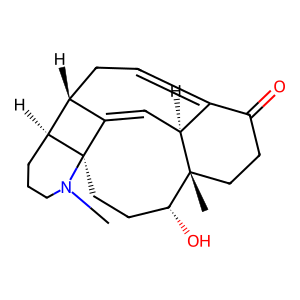
\includegraphics{../graphics/morphine_structure.png}

}

\subcaption{\label{fig-morphin}Cấu trúc hóa học của morphin}

\end{minipage}%
%
\begin{minipage}{0.50\linewidth}

\centering{

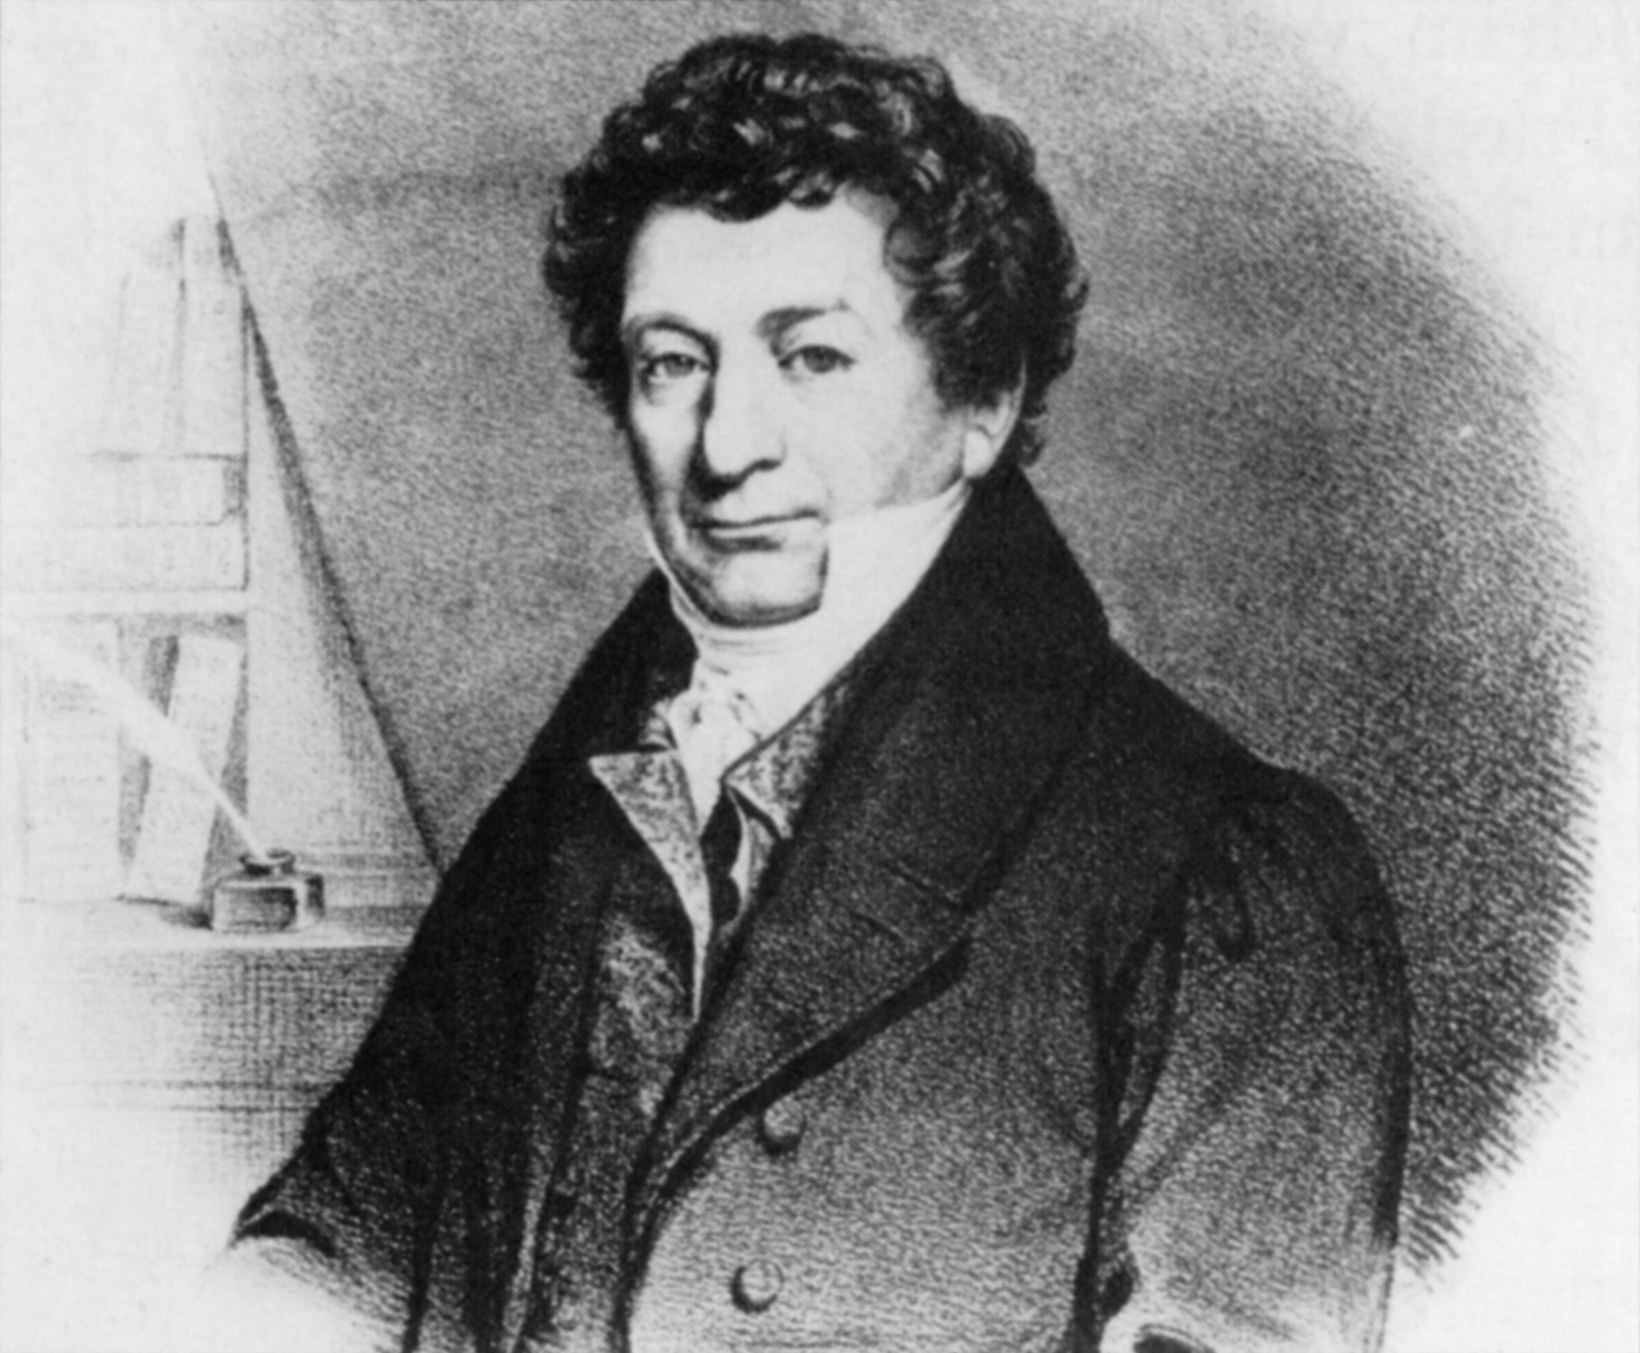
\includegraphics{../graphics/Friedrich_Wilhelm_Adam_Sertuerner.jpg}

}

\subcaption{\label{fig-Adm-Seruerner}Friedrich Serturner}

\end{minipage}%

\caption{\label{fig-morphine}Năm 1804, dược sĩ người Đức Friedrich
Serturner đã phân lập được morphine từ nhựa cây thuốc phiện
(\emph{Papaver somniferum}). Đây được coi là hợp chất đầu tiên phân lập
từ thực vật và hãng dược phẩm Merk đã bắt đầu thương mại hóa hợp chất
này từ năm 1827. Tên của hoạt chất này theo tiếng Latin là
\emph{morphium} biến thể từ tên của một vị thần giấc mơ trong tiếng Hy
lạp \emph{Morpheus}.}

\end{figure}%

Các hợp chất có hoạt tính sinh học từ thực vật là nhóm các chất chuyển
hóa bậc hai và có tác dụng dược lý cũng như có thể gây độc trên động vật
và con người. Quá trình sinh tổng hợp các chất chuyển hóa bậc hai trong
thực vật diễn ra như là kết quả của quá trình trao đổi chất với nguyên
liệu đầu vào gồm các hợp chất bậc một liên quan đến sự tăng trưởng và
phát triển của thực vật. Do đó, các hoạt chất có hoạt tính sinh học
thường được coi là sản phẩm phụ của quá trình chuyển hóa tế bào thực
vật.\textsuperscript{3} Mặc dù không đảm nhận vai trò dinh dưỡng nhưng
các hợp chất này cũng có thể đóng vai trò quan trọng đảm bảo sự phát
triển của thực vật, ví dụ.\textsuperscript{4}:

\begin{itemize}
\item
  Quá trình quang hợp, các flavonoid đóng vai trò như các hợp chất chặn
  gốc tự do;
\item
  Terpenoid tạo ra mùi hương cho hoa để thu hút các loài đến thụ phấn
  hoặc hương vị cho quả để phát tán hạt;
\item
  Các alkaloid thường tạo ra độc tính để xua đuổi hoặc ngăn chặn côn
  trùng và các động vật ăn cỏ.
\end{itemize}

Cây lương thực và thực phẩm đều tạo ra các hợp chất có hoạt tính sinh
học nhưng nồng độ thấp hơn so với cây thuốc hoặc cây có
độc.\textsuperscript{5,6} Các nghiên cứu đều xác nhận rằng các hợp chất
chuyển hóa bậc hai này có tác dụng bảo vệ sức khỏe con người và là yếu
tố chính của một chế độ ăn uống lành mạnh. Chúng cũng có tác dụng hữu
ích trong ngăn ngừa các bệnh tim mạch, viêm nhiễm, rối loạn lipid và béo
phì.\textsuperscript{7} Ví dụ nổi bật nhất chính là vai trò của hợp chất
tự nhiên trong giải thích bí ẩn về sức khỏe của người Pháp. (French
Paradox) Hiện tượng này được các nhà dịch tế người Pháp phát hiện ra vào
thập niên 1980 khi tỷ lệ tử vong do bệnh tim mạch và vành tại Pháp thấp
mặc dù chế độ ăn giàu chất béo bão hòa và cholesterol. Qua nhiều nghiên
cứu, giả thuyết được nhiều nhà khoa học đồng tình là do thói quen sử
dụng rượu vang. Trong rượu vang có nhiều flavonoids, đây là nhóm hợp
chất tự tự nhiên có vai trò ức chế quá trình oxy hóa các lipoprotein
khối lượng phân tử bé (Low density lipoprotein), ngăn ngừa quá trình
lipid bị oxy hóa và giảm thiểu hình thành xơ vữa mạch. Ngoài ra, rượu
vang đỏ cũng chứa nhiều polyphenol từ vỏ quả nho cũng có tác dụng chống
oxy hóa mạnh. Tuy nhiên, điều này là chưa đủ bằng chứng để giải thích.
Các nhà khoa học cũng đồng thuận rằng sự kết hợp giữa uống rượu vang và
chế ăn ăn Đại Trung Hải mới tạo ra được hiệu quả thực sự. Nồng độ
Catechin trong huyết tương- một flavonoid có tác dụng chống oxy hóa
mạnh- của chế độ ăn có trái cây, rau không rượu cao gấp ba lần khi so
với chế độ ăn không trái cây, rau hay rượu và cao gấp bốn lần chế độ ăn
có rượu vang đỏ nhưng không có rau và trái cây.\textsuperscript{8,9} Từ
đó cho thấy hợp chất từ tự nhiên là một thành phần quan trọng trong chế
độ ăn uống của con người và quá trình chiết xuất các hợp chất này cần
được quan tâm.

\section{1.2 Phân loại các hợp chất từ tự
nhiên}\label{phuxe2n-loux1ea1i-cuxe1c-hux1ee3p-chux1ea5t-tux1eeb-tux1ef1-nhiuxean}

Cách phân loại các hoạt chất có hoạt tính sinh học từ thực vật có thể
dựa trên các tiêu chí như lâm sàng, độc tính, dược lý hoặc thực vật học.
Nhìn chung, mối liên hệ giữa cấu trúc và tác dụng sinh học nhiều khi
không rõ ràng, thâm chí, các loài mặc dù có mối liên hệ di truyền nhưng
tạo ra các phân tử có hoạt tính sinh học không giống nhau, dẫn tới cách
phân loại trên không đạt hiệu quả như mong đợi.\textsuperscript{3} Cách
phân loại dựa trên cấu trúc hóa học và con đường sinh hóa sẽ tốt hơn.
Theo Croteau \emph{et al.}\textsuperscript{10} và Taiz \emph{et
al.},\textsuperscript{11}, các hợp chất có hoạt tính sinh học từ các
nguồn thực vật có thể phân loại thành:

\begin{itemize}
\item
  Terpen và terpenoid (khoảng 25.000 hợp chất) được tạo ra bởi con đường
  acid mevalonic và non-mevalonate (MEP);
\item
  Alkaloid (khoảng 12.000 hợp chất) được sản xuất thông qua con đường
  acid shikimic và;
\item
  Hợp chất phenolic (khoảng 8000 hợp chất) được sản xuất bởi con đường
  acid malonic và acid shikimic.
\end{itemize}

\subsubsection{1.2.1 Nhóm Terpenes}\label{nhuxf3m-terpenes}

Trong số các hợp chất tự nhiên, terpenoid chiếm nhóm lớn nhất với cấu
trúc hóa học được cấu thành từ các isoprene. Khoảng 25.000 hợp chất được
xác định thuộc nhóm này có vai trò chính bảo vệ thực vật khỏi các tác
nhân gây hại đồng thời cũng có nhiệm vụ thu hút côn trùng tới thụ
phấn.\textsuperscript{12} Với y học và công nghệ sinh học, các terpenoid
có tác dụng dược lý rộng từ chống viêm, kháng khuẩn tới ức chế tế bào
ung thư hay kích thích tra đổi chất. Có hai con đường chính để sinh tổng
hợp ra terpen trong thực vật gồm con đường acid mevalonic và con đường
không acid mevalonic thông qua deoxyxylulose phosphate. Con đường acid
mevalonic được tiến hành trong tế bào chất và ty thể của tế bào thực
vật, ở đó, các hợp chất khác nhau được tổng hợp cụ thể gồm sterol,
sesquiterpenes và ubiquinones.\textsuperscript{13} Trong khi con đường
không acid mevalonic thông qua deoxyxylulose phosphate được diễn ra tại
plastid của tế bào thực vật và điều chế các hợp chất như hemi-, mono-,
sesqui- và diterpenes, ngoài ra carotenoid và nhóm phytol của chất diệp
lục.\textsuperscript{14}\\

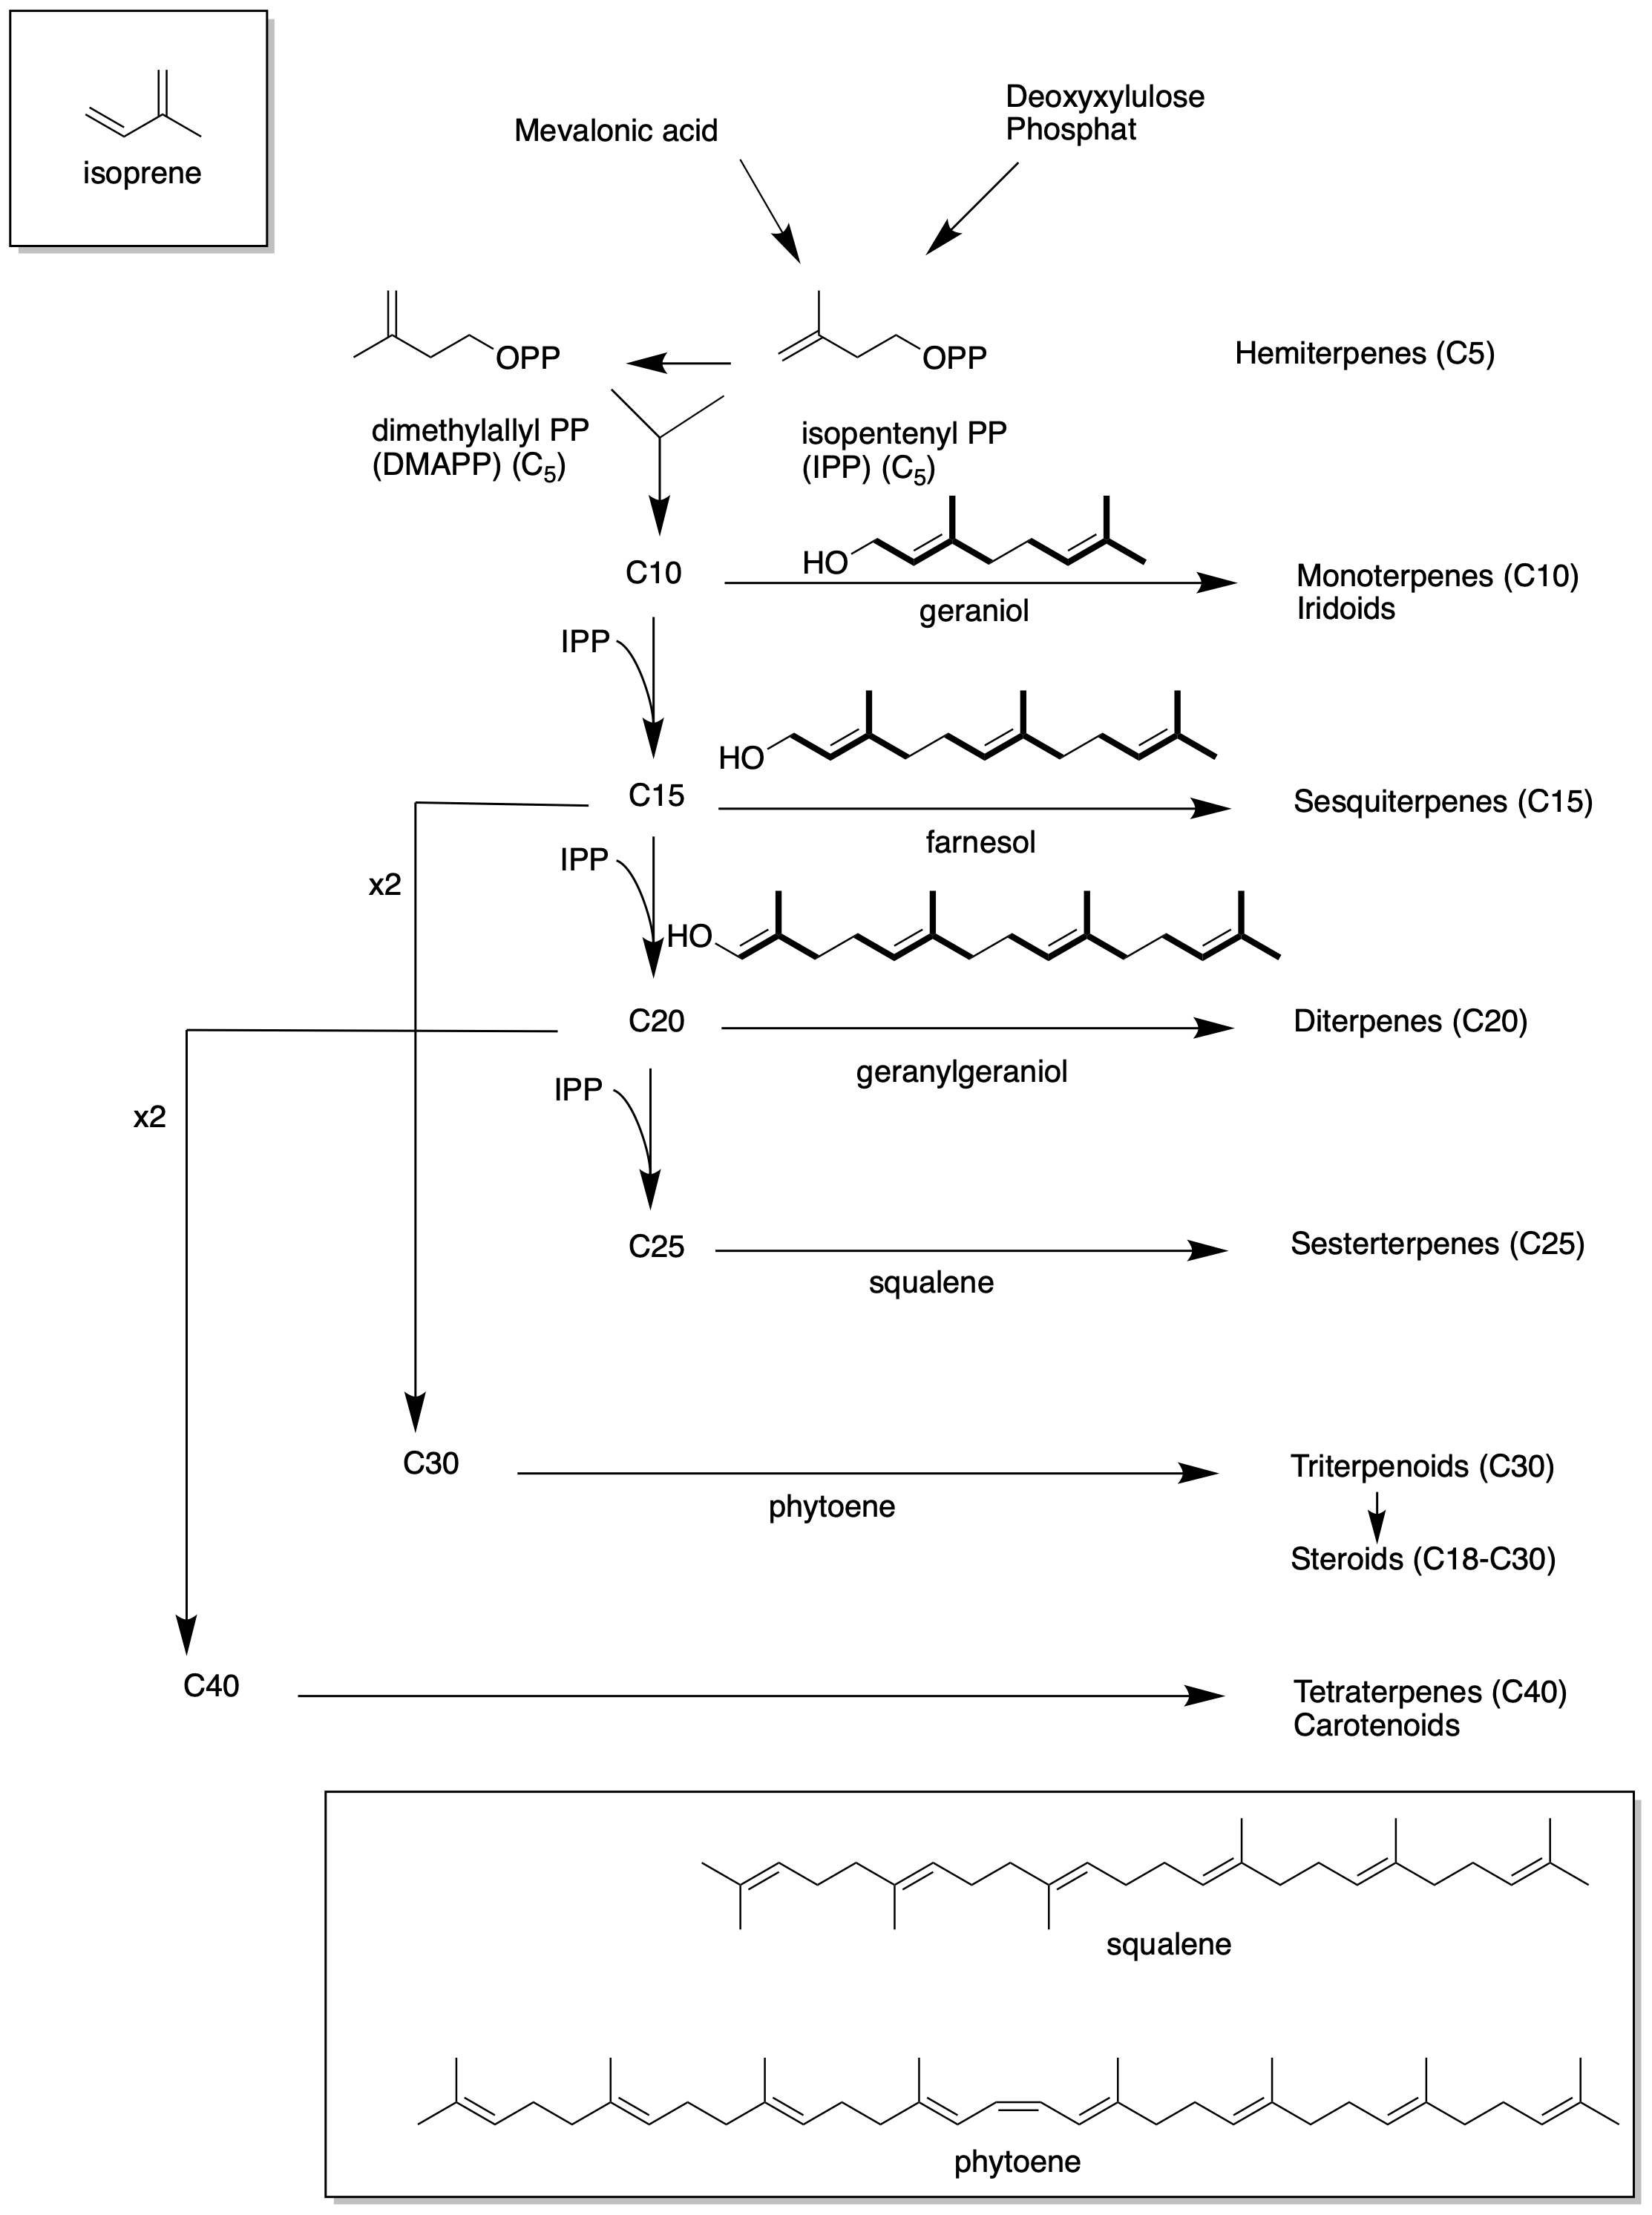
\includegraphics{../graphics/isoprene and pathway.png}\{\#fig:isoprene
and pathway\}

Nếu dựa trên số đơn vị isoprene, terpen có thể chia thành các nhóm nhỏ
hơn gồm các hemi-, mono-, sesqui-, di-, sester-, triterpen. Nhóm
monoterpen là thành phần chính trong các tinh dầu với đặc trưng là nhóm
mạch hở geraniol, linalool và myrcene hoặc mạnh vòng camphor, menthol,
limonene và pinene. Với nhiệt độ sôi cao hơn, nhóm diterpen mặc dầu có
thể thu được bằng phương pháp cất kéo hơi nước giống monoterpe nhưng
không bay hơi ở nhiệt độ phòng và coi là thành phần của nhựa thực vật.
Nhóm sesquiterpene với ba đơn vị isoprene thường là ở dạng hai hoặc ba
vòng. Farnesol là một sesquiterpene mạch hở quan trọng của quá trình
tổng hợp terpene. Arteether là sesquiterpene lactone có nguồn gốc từ
\emph{Artemisia annua} (Thanh hao hoa vàng) có tác dụng điều trị sốt
rét. Triterpenes với số Carbon chủ yếu bằng 30 tạo thành từ sáu đơn vị
isoprene thông qua quá trình đóng vòng squalene. Những hợp chất như vậy
có điểm nóng chảy cao hơn, không màu, ở dạng rắn và chủ yếu được tìm
thấy trong nhựa thực vật, lớp bần, và cu-tin. Các Steroid, saponin và
glycoside tim thuộc nhóm này thường có hoạt tính sinh học mạnh. Từ hạt
của \emph{Azadirachta indica} (cây Nem, sầu đâu) chiết được nimbolide có
khả năng diệt tế bào ung thư vú mạnh thông phân giải protein.
Cucurbitacin được phân lập từ họ Cucurbitaceae năm 1954 tạo ra vị đắng,
có tác dụng diệt côn trùng và ức chế tế bào ung thư. Các steroid thực
vật là dạng chuyển đổi của triterpene có chứa hệ thống vòng bốn của
lanosterol nhưng thiếu ba nhóm methyl tại vị trí C4 và C14. Diosgenin là
nguồn nguyên liệu quan trọng của công nghiệp hóa dược, ước tính 60\%
thuốc nhóm steroid như thuốc chống viêm cortison, progesterone,
hydrocortison hay progesteron, testrosteron được bán tổng hợp từ hoạt
chất này. Diosgenin có thể chiết từ các loài thuộc chi Dioscorea (Họ
Dioscoreaceae).\textsuperscript{15} Khi gắn thêm mạch đường vào
triterpen sẽ tạo thành nhóm phổ biến khác trong thực vật là triterpen
saponin. Một số tác dụng của dược liệu đã được chứng minh là do nhóm
triterpen saponin tạo ra như \emph{Glycerrhiza glabra} (cam thảo),
\emph{Panax ginseng} (nhân sâm), \emph{Hedera helix} (thường xuân).
Glycyrrhizins là dạng muối của amoni và canxi của acid glycyrrhizic, và
trên thang đo độ ngọt, chúng ngọt hơn 50--100 lần so với
đường.\textsuperscript{16}

\subsubsection{1.2.2 Nhóm Alkaloids}\label{nhuxf3m-alkaloids}

Các alakaloids là những hợp chất dị vòng có chứa nitơ thường có hoạt
tính sinh học mạnh và vị đắng. Hiện tại, 12.000 alkaloid được phân lập
và xác định cấu trúc hóa học từ khoảng 150 họ. Các họ thực vật bậc cao
quan trọng với ngành dược gồm Papaveraceae, Apocynaceae, Ranunculaceae,
Fabaceae, Rubiaceae, Solanaceae, và Rutaceae trong khi thực vật bậc thấp
và nấm ít phổ biến hơn (alkaloid nấm cựa gà).\textsuperscript{17} Về cấu
trúc hóa học, các alakaloid trong tự nhiên tạo dạng muối với một số acid
hữu cơ như acid malic, oxalic, lactic, citric, tannic, tartaric. Với một
số alakaloid dạng base yếu như nicotin sẽ ở dạng tự do. Một số alakaloid
ở dạng glycoside khi gắn với một số mạch đường tạo thành tư các đường
đơn như galactose, glucose và rhamnose như solanine. Chúng cũng ở dạng
amid (piperine) hay dạng ester với acid hưu cơ (cocaine và
atropine).\textsuperscript{18} Nhiều bộ phận khác nhau của thực vật chứa
alakaloid chẳng hạn trong hạt cây \emph{Strychnos nuxvomia} (mã tiền)
chứa nhiều strychnine, brucine, trong rễ cây \emph{Coptis chinensis}
(hoàng liên bắc) chứa berberin, trong vỏ thân cây \emph{Holarrhena
pubescens} (mộc hoa trắng, mực hoa trắng) có chứa conessin. Alkaloid
xuất hiện trong cây hai lá mầm so với cây một lá mầm. Thực vật chứa
alakaloid thường được quan tâm do tác dụng dược lý mạnh và bản thân các
alakaloid cũng có tác dụng sinh học. Ví dụ phổ biến nhất là vinblastine
chiết từ \emph{Catharanthus roseus} (cây dừa can) được sử dụng làm thuốc
điều trị ung thư như ung thư phổi tế bào không nhỏ, ung thư não, u ác
tính hay ung thư tinh hoàn. Thuốc giảm đau morphine và codeine phân lập
từ nhựa cây \emph{Papaver somniferum} (thuốc phiện, anh túc). Thuốc giãn
cơ tubocurarine sử dụng trong phẫu thuật được phân lập từ vỏ cây
\emph{Chondrodendron tomentosum}. Caffeine từ quả cà phê, trà cùng với
nicotin từ thuốc lá có ảnh hưởng đến thần kinh trung ương được sử dụng
trong chế phẩm nhai, hút.\textsuperscript{19} Mối liên hệ giữa cấu trúc
hóa học, sinh tổng hợp trong họ thực vật và tác dụng sinh học của các
alakaloid cũng tương đối là rõ ràng. Ví dụ nhóm alkaloid tropane được
tìm thấy nhiều trong họ Solanaceae ở \emph{Atropa belladonna},
\emph{Datura spp.}, và \emph{Hyoscyamus niger} đều thể hiện tác dụng
kháng cholinergic, làm giảm co thắt cơ trơn, giảm đau và tăng tiết. Bên
cạnh tác dụng điều trị, alakaloid cũng gây ra độc tính và thường xuất
hiện trong thực phẩm và thực phẩm bổ sung. Nổi bật là các alkaloid nhóm
pyrrolizidine xuất hiện trong ba họ thực vật Asteraceae (họ cúc),
Boraginaceae và Leguminosae (Fabaceae) có thể gây độc trên phổi và gan.
Năm 1997, FDA Hoa kỳ đã công bố quy định hướng dẫn về thực hành sản xuất
tốt (GMP) theo đó các nhà sản xuất cần phải cải thiện sản phẩm để giảm
thiểu sự xuất hiện của nhóm pyrrolizidine.

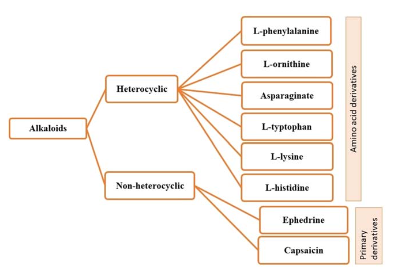
\includegraphics{../graphics/Classification of alkaloids.png}\{\#fig:Classification
of alkaloids width=``\textbackslash textwidth''\}

\subsubsection{1.2.3 Polyphenols}\label{polyphenols}

Polyphenol là các chất chuyển hóa bậc hai trong thực vật. Với gần 8000
hoạt chất đã được phân lập và xác định cấu trúc. Chúng có thể phân thành
các nhóm nhỏ hơn dựa trên số vòng phenol và các nhóm thế. Các nhóm nhỏ
hơn bao gồm các acid phenolic phenolic (acid hydroxycinnamic và acid
hydroxybenzoic), flavonoid (flavonol, flavanol, flavanone, flavon,
proanthocyanidin và isoflavone), tanin, stilben và
lignan.\textsuperscript{4,20} Đơn vị cấu tạo của polyphenol từ một vòng
thơm gắn với một nhóm OH hoặc nhóm carbonyl.\textsuperscript{21} Hầu
hết, các hợp chất polyphenolic được sinh tổng hợp thông qua con đường
shikimate như flavonoid, stilben, xanthones, nhưng đôi khi thông qua con
đường polyketide ví dụ orcinol và quinon.\textsuperscript{22} Các
polyphenol có thể tập trung tìm thấy trong các bộ phận của thực vật như
lá, vỏ cây, hoa, và quả.\textsuperscript{23} Với thực vật, các
polyphenol có vai trò tạo màu sắc, mùi vị và tạo nguồn dinh dưỡng tại
quả.\textsuperscript{24}.\\

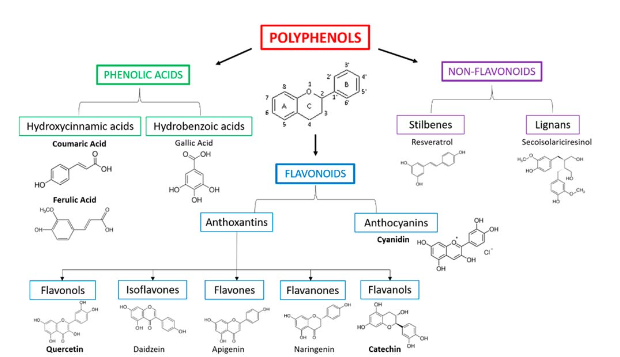
\includegraphics{../graphics/Classification of polyphenols.png}\{\#fig:Classification
of polyphenol width=``\textbackslash textwidth''\}

Nhóm polyphenol quan trọng đầu tiên cần đề cập tới là các flavonoid. Đây
là nhóm hợp chất được tạo bởi hai vòng pheonlic nối với nhau thông qua
một cầu 3 carbon và thường ở dạng glycoside. Bất cứ hợp chất flavonoid
nào đều có hoạt tính chống oxy hóa. Ngoài ra khả năng chống viêm và ức
chế tế bào ung thư cũng là tính chất đặc trưng của nhóm này. Các khung
isoflavone hay còn gọi là phytoestrogen (thực vật nữ sắc tố) có thêm tác
dụng giống như hormon nội sinh estrogene và sử dụng nhưng thực vật chứa
nhóm này sẽ có lợi trong quá rối loạn quanh và hậu mãn kinh. Nguồn cung
cấp isoflavone thường đến tự họ Fabaceae (họ Đậu) như đậu tương, đỗ
xanh, đỗ đen. Một số hoạt chất đại diện cho nhóm này như genistein và
daidzein được các nhà khoa học quan tâm để phân lập, làm giàu hay làm
chất chuẩn để giám sát chất lượng sản phẩm.\textsuperscript{25}\\
Tanin là hợp chất cao phân tử có cấu trúc hóa học phức tạp thuộc nhóm
polyphenol. Dựa trên cấu trúc hóa học, tanin chia thành hai nhóm gồm
ngưng tụ và nhóm thủy phân. Nhóm ngưng tự là một cao phân tử chứa các
đơn vị flavonoid trong cấu trúc của chúng trong khi nhóm thủy phân được
cấu tạo từ trung tâm là một đường đơn (thường là glucose) tạo liên kết
của các nhóm OH với dẫn xuất của catechin hoặc acid pheonlic. Độ tan của
tanin phụ thuộc vào kích thước phân tử. Tanin thường sẽ cản trở quá
trình hấp thu dinh dưỡng do khả năng tạo liên kết với protein và khoáng
chất trong khi tanin có khối lượng phân tử lớn hơn sẽ có khả năng làm
săn se ứng dụng trong điều trị một số bệnh như tiêu chảy, tăng tiết dịch
hoặc chảy máu. Tanin xuất hiện trong hầu hết thực vật nhưng họ thực vật
được quan tâm trong dược liệu gồm Fagaceae (họ Sồi) và Polygonaceae (Họ
rau răm).\textsuperscript{26}\\
Phân nhóm có hoạt tính sinh học mạnh thuộc phenol cuối cùng đề cập là
các lignan. Đây là nhóm với cấu trúc hóa học tạo thành từ các Lignans
chứa các nhóm chức năng khác nhau và bao gồm hai đơn vị phenylpropanoid
ghép nhau và thường có 18 carbon. Các hợp chất này xuất hiện trong màng
tế bào và thường tan trong dung môi hữu cơ không phân cực. Lignans giống
như isoflavone xếp vào nhóm các hợp chất phytoestrogen. Chúng xuất hiện
nhiều trong thực phẩm hàng ngày như lúa mạch, lúa mì, hạt vừng. Các hoạt
chất thường hay gặp trong chế ăn hàng ngày của con người là
secoisolariciresinol, matairesinol, lariciresinol, pinoresinol và
syringaresinol. Khi ăn vào, secoisolariciresnol và matairesinol được
chuyển đổi thành enterodiol và enterolactone (hai lignan do động vật có
vú sinh tổng hợp ra) nhờ các enzym của vi sinh vật trong ruột kết.
Enterodiol và enterolactone giúp cơ thể bảo vệ chống lại các bệnh tim
mạch, ung thư vú và ung thư tiền liệt tuyến thể liên quan tới hormon.
Chế độ ăn giàu lignan cũng giúp tỷ lệ ung thư thấp, điều này đã được
công bố trong nghiên cứu tại Đan mạch trên 875 phụ nữ mãn kinh. Các phụ
nữ ăn nhiều ngũ cốc nguyên hạt sẽ có nồng độ enterolactone trong máu cao
hơn đang kế. Trong khi đó, nồng độ enterolactone cao sẽ tỷ lệ nghịch với
bệnh tim mạch.\textsuperscript{27}

\subsubsection{1.2.4 Nhóm chất khác}\label{nhuxf3m-chux1ea5t-khuxe1c}

Protein thực hiện một vai trò cực kỳ quan trọng đối với cuộc sống. Khi
protein hấp thụ vào cơ thể từ mô ruột sẽ cung cấp các khối cơ bản để xây
dựng cấu trúc cơ thể. Nhưng cũng có nhưng protein đóng vai trò như một
hoạt chất cao phân tử có hoạt tính sinh học.\textsuperscript{28} Các
protein này khi hấp thu qua đường tiêu hóa sẽ không bị thủy phân mà hấp
thu vào máu và duy trì chức năng đặc biệt trong cơ thể. Ví dụ, ricin
chiết xuất từ hạt cây \emph{Ricinus communis} (đậu thầu dầu) thuộc họ
Euphorbiaceae (Họ Thầu dầu) gây độc tính cấp trên cơ thể với triệu chứng
ói ra máu, hoại tử, suy thận và trụy tim mạch.\textsuperscript{29}
Glycoside là một nhóm lớn gồm aglycone liên kết với phần đường trong đó
aglycone là nhiều loại chất chuyển hóa thứ cấp khác nhau. Glycoside
Cyanogen, glycoside tim, glycoside anthraquinone, saponin và
glucosinolate là một số nhóm glycoside chính. Flavonoid cũng được tìm
thấy dưới dạng glycoside. Sừ dụng theo đường tiêu hóa, các glycoside bị
thủy phân ở phần ruột kết và các glycoside kỵ nước hơn (aglycone) có thể
được hấp thụ.\textsuperscript{30} Các hợp chất có tác dụng sinh học mạnh
thuộc nhóm này cần đề cập đầu tiên là các glycoside tim với phần
aglycones có cấu trúc là steroid. Các hoạt chất nhóm này có thể ức chế
các bơm Na+/K+-ATPase hoạt động trên màng tế bào cơ tim. Digoxin chiết
suất từ cây \emph{Digitalis spp.} (mao địa hoàng) hoặc Neriolin từ lá
cây \emph{Nerium Oleander} (lá trúc đào) có tác dụng trên tim điều trị
một số bệnh như chậm nhịp tim. Nhóm tiếp theo là các glycoside cyanogen
có gốc aglycone là các acid amin.\textsuperscript{31} Suy giáp có thể
xuất hiện nếu sử dụng cao chiết có nhóm hoạt chất này do có thể cản trở
việc hấp thu Idod. Nếu các acid amin trong phần alycone có chứa lưu
huỳnh thì các hoạt chất này thường sẽ có mùi hăng. Tại cấp độ tế bào,
chúng giúp giảm độc tính của các chất gây ung thư tại gan thông qua một
quá trình phức tạp ảnh hưởng đến các cytochrom P450. Nhóm cuối cùng là
các saponin với aglycone thuộc nhóm triterpen. Các saponin có đặc tính
nhũ hóa liên quan đến phần đường có khối lượng phân tử lớn thân nước và
phần aglycone kỵ nước.

\subsection{1.3 Tầm quan trọng của quá trình chiết
xuất}\label{tux1ea7m-quan-trux1ecdng-cux1ee7a-quuxe1-truxecnh-chiux1ebft-xuux1ea5t}

Quá trình chiết xuất là giai đoạn quan trọng trong nghiên cứu và phát
triển sản phẩm từ dược liệu khi tác động đáng kể đến kết quả cuối cùng.
Sản phẩm quá trình chiết xuất là hỗn hợp các hoạt chất với cấu trúc hóa
học đa dạng với tiềm năng tác dụng sinh học khác nhau. Nồng độ từng hoạt
chất trong hỗn hợp chiết được là khác nhau. Trong trường hợp nồng độ
hoạt chất quan tâm có nồng độ thấp trong dược liệu có thể cần thêm quá
trình xử lý để làm giàu hàm lượng. Khi đó, công nghệ sản xuất phức tạp
và thường dẫn tới chi phí tăng cao hơn ban đầu.\textsuperscript{32} Mặc
dù các kỹ thuật sắc ký và phương pháp quang phổ cũng đóng góp vai trò
lớn trong phân lập và xác định cấu trúc hóa học của các hoạt chất nhưng
quá trình chiết xuất đòi hỏi tới hai phần ba về thời gian, nguồn nhân
lực và chi phí của một dự án phát triển sản phẩm từ dược liệu thành
công.\textsuperscript{33} Nhưng khó khăn về đa dạng thành phần trong
dược liệu cộng thêm lựa chọn được hợp chất có tác dụng sinh học đích đã
thúc đẩy các công nghệ chiết xuất mới để tối ưu hóa quy trình nghiên cứu
và sản xuất. Hiện nay, nhiều nhà nghiên cứu đang phát triển các phương
pháp khác nhau để sàng lọc các cao chiết có hoạt tính sinh học từ các
nguồn tự nhiên ứng dụng trong phòng ngừa và điều trị các bệnh khác nhau
của con người. Hiệu quả của các hỗn hợp này khi tương tác với các đích
phân tử sinh học bao gồm enzyme và protein sẽ cung cấp các bằng chứng
cho phép sử dụng cao chiết từ thực vật trong các liệu pháp điều
trị.\textsuperscript{34} Do đó, với mục đích này, chiết xuất các phân tử
có hoạt tính sinh học từ các nguồn thực vật cùng xây dựng tiêu chuẩn
kiệm nghiệm bao gồm định tính và định lượng là rất quan trọng để phát
triển thuốc mới từ dược liệu.\textsuperscript{35} Theo UNESCO, 80\% dân
số chủ yếu đang sinh sống tại các nước đang phát triển phụ thuộc vào sử
dụng các sản phẩm từ dược liệu để chăm sóc sức khỏe.\textsuperscript{36}
Với hàng nghìn các hợp chất hóa học có thể hiện diện trong dược liệu,
phổ tác dụng của sản phẩm từ dược liệu rất đa dạng từ điều trị các bệnh
truyền nhiễm cho tới hoạt tính sinh học có lợi như chống oxy hóa, kháng
viêm, kháng khuẩn, chống ung thư, giảm đau.\textsuperscript{37} Từ cao
chiết từ thực vật, ngàngh công nghiệp thực phẩm đang tập trung sản xuất
và phát triển các sản phẩm bảo vệ sức khỏe với sự quan tâm ngày càng
tăng của người tiêu dùng. Nhìn chung, các sản phẩm này bao gồm nhiều
loại với tỷ lệ các hợp chất có hoạt tính sinh học khác
nhau.\textsuperscript{38} Chúng có thể được gắn nhãn mác khác nhau trên
thị trường như sản phẩm bảo vệ sức khỏe, thực phẩm chức năng, thực phẩm
bổ sung. Tuy nhiên, các sản phẩm này có thể hiểu là một sản phẩm mới
trong đó thành phần được cấu tạo từ các hợp chất có hoạt tính sinh học,
tác dụng từng hợp chất riêng lẻ có thể giống nhau hoặc khác
nhau.\textsuperscript{39} Plaza \emph{et al.}\textsuperscript{40} đã đề
cập tới ba yếu tố chính cần phải có trong sản phẩm bảo vệ sức khỏe từ
thực vật. Trước hết, tác dụng của chúng phải khác so với chế độ ăn thông
thường. Thứ hai, chúng phải có dữ liệu tin cậy về việc không có bất kỳ
tác dụng có hại nào. Và cuối cùng, chúng sẽ có lợi trong việc giảm nguy
cơ tiến triển của bệnh lý và cũng sẽ giúp cải thiện chức năng sinh lý.
Do đó, các hoạt chất có hoạt tính sinh học như kháng vi-rút, chống oxy
hóa, hạ huyết áp, chống tiểu đường, \(\ldots\) phải được chiết xuất từ
nguồn thực vật sau đó sử dụng trong việc xây dựng công thức bào chế các
sản phẩm bảo vệ sức khỏe khác nhau vì thực tế không có một hoạt chất
toàn năng. Điều cần lưu tâm trong phát triển các sản phẩm dạng này cần
phân biệt giữa tác dụng và chỉ định. Các sản phẩm bảo vệ sức khỏe có thể
dược chỉ định dựa trên tác dụng ví dụ giúp giảm cholesterol máu, chống
ung thư, giảm tình trạng không dung nạp đường sữa, hoặc giảm tiêu chảy
nhanh hơn.\textsuperscript{41--43} Trên thị trường, chúng có thể bán
dưới dạng sản phẩm thông thường như bánh, đồ uống hay gói ngũ cốc hoặc
áp dụng bào chế của thuốc để chuyển dạng. Trong đó, dạng đồ uống thường
tiện lợi hơn do dễ xử lý, chế biến và pha chế so với các loại khác.

\subsection{1.4 Một số dung môi phổ biến dùng trong chiết
suất}\label{mux1ed9t-sux1ed1-dung-muxf4i-phux1ed5-biux1ebfn-duxf9ng-trong-chiux1ebft-suux1ea5t}

Các kỹ thuật thông thường để chiết xuất dược liệu bao gồm chiết xuất
lỏng-lỏng hoặc rắn-lỏng, chiết xuất Soxhlet, ngâm và cất kéo hơi nước.
Trong đó phương pháp chiết sử dụng Soxhlet được coi là truyền thống và
lâu đời nhất. Điểm chung các phương pháp này đều phụ thuộc phần lớn lựa
chọn đúng dung môi chiết xuất với mục tiêu thu được hợp chất mong muốn
và cải thiện hiệu suất dựa trên tác động vật lý như nhiệt và/hoặc trộn.
Tại thời điểm hiện tại, lý thuyết lựa chọn dung môi trong chiết xuất
dược liệu chỉ mang tính tương đối. Bảng
\hyperref[tab:typesux5cux2520ofux5cux2520solvent]{{[}tab:types of
solvent{]}} dựa trên kinh nghiệm thể hiện nhóm hoạt chất kỳ vọng thu
được từ dung môi chiết xuất. Các dung môi này phổ biến trong nghiên cứu
và thường được áp dụng triển khai trong công nghiệp. Dung môi nước
thường được ưu tiên sử dụng hơn nhưng sẽ hao tốn về năng lượng trong quá
tình chiết xuất. Khi sử dụng các dung môi, yêu cầu bắt buộc người lao
động phải có kỹ năng cao vận hành thiết bị, xử lý sự cố cũng như giảm
thiểu rủi ro trong quá trình sản xuất. Thêm nữa, áp dụng nội dung trong
bảng cũng khá phức tạp nguyên nhân trong dược liệu có thể chứa hàng
trăm, hàng ngàn hoạt chất. Đặc biệt nhóm cao phân tử như tinh bột,
polysacharride, protein có thể tạo lớp màng gây cản trở quá trình chiết
suất.

Gần đây một số thiết bị mới ra đời áp dụng tiến bộ về công nghệ để chiết
suất, có thể kể ra như chiết xuất siêu tới hạn, chiết lỏng có áp suất,
siêu âm và vi sóng. Ngoài ra, quá trình chiết xuất có thêm sự hỗ trợ bởi
xung điện trường và chiết xuất ohmic. Các phương pháp chiết xuất mới về
cơ bản được sử dụng để tăng cường giải phóng các hợp chất từ tế bào thực
vật. Hơn nữa, việc giảm sử dụng dung môi hữu cơ trong các phương pháp
này làm cho chúng còn được gọi là phương pháp chiết xuất xanh. Một đặc
trưng nữa của các phương pháp này làm giảm thời gian chiết xuất dẫn đến
năng suất tốt hơn và chất lượng sản phẩm cuối cao hơn. Và dự đoán trong
vài năm tới, những công nghệ này có thể phổ biến hơn do cách tiếp cận
thân thiện với môi trường thúc đẩy ngành công nghiệp chế tạo dụng cụ đề
tăng năng suất và giảm chi phí.

\subsection{1.5 Phân đoạn bằng phương pháp chiết
lỏng-lỏng}\label{phuxe2n-ux111oux1ea1n-bux1eb1ng-phux1b0ux1a1ng-phuxe1p-chiux1ebft-lux1ecfng-lux1ecfng}

Để thu được sản phẩm có chất lượng hơn, mẫu sau khi chiết xong có thể xử
lý trước bằng phương pháp phân đoạn lỏng-lỏng. Đây là kỹ thuật tiền xử
lý được sử dụng phổ biến nhất trong giai đoạn hiện tại. Quá trình phân
đoạn có thể tách một nhóm chất ra khỏi mẫu ban đầu dựa trên độ phân cực
của dung môi không đồng tan. (Hình
\hyperref[fig:Liquid-Liquidux5cux2520Extractor]{1.4}) Nguyên lý phương
pháp dựa trên một hoạt chất có xu hướng phân bố nhiều vào lớp dung môi
có độ phân cực gần với hoạt chất hơn. Hệ quả là, hoạt chất có thể tách
khỏi mẫu nền. Danh mục các dung môi không đồng tan với nhau được biểu
diễn trong hình
\hyperref[fig:Solventux5cux2520miscibilityux5cux2520chart]{1.5}. Hiệu
quả của quá trình chiết phân đoạn lỏng lỏng ngoài lựa chọn hai dung môi
không đồng tan, còn ảnh bởi pH, tỷ lệ giữa hai pha, số lần phân đoạn.

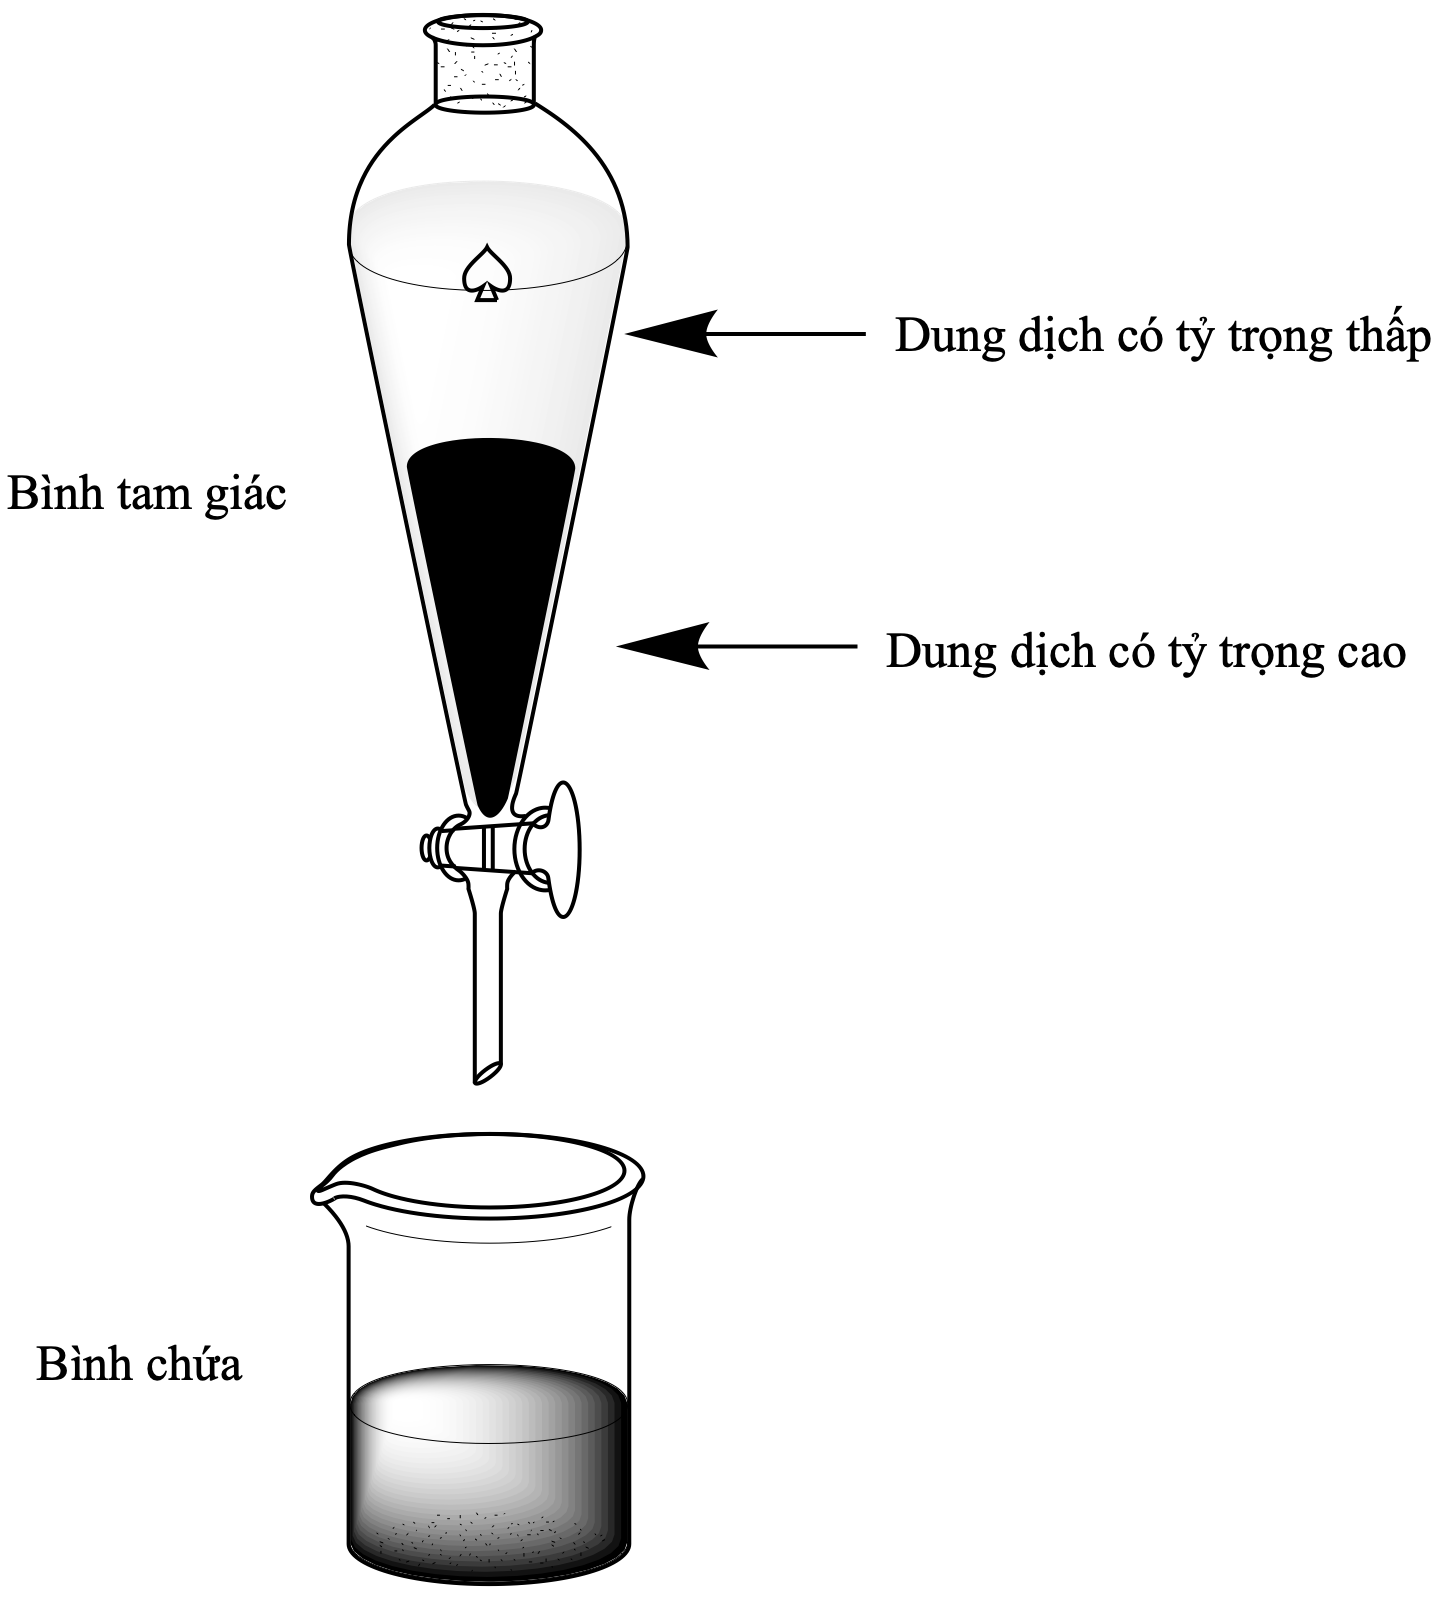
\includegraphics{../graphics/Liquid-Liquid Extractor.png}\{\#fig:Liquid-Liquid
Extractor\}

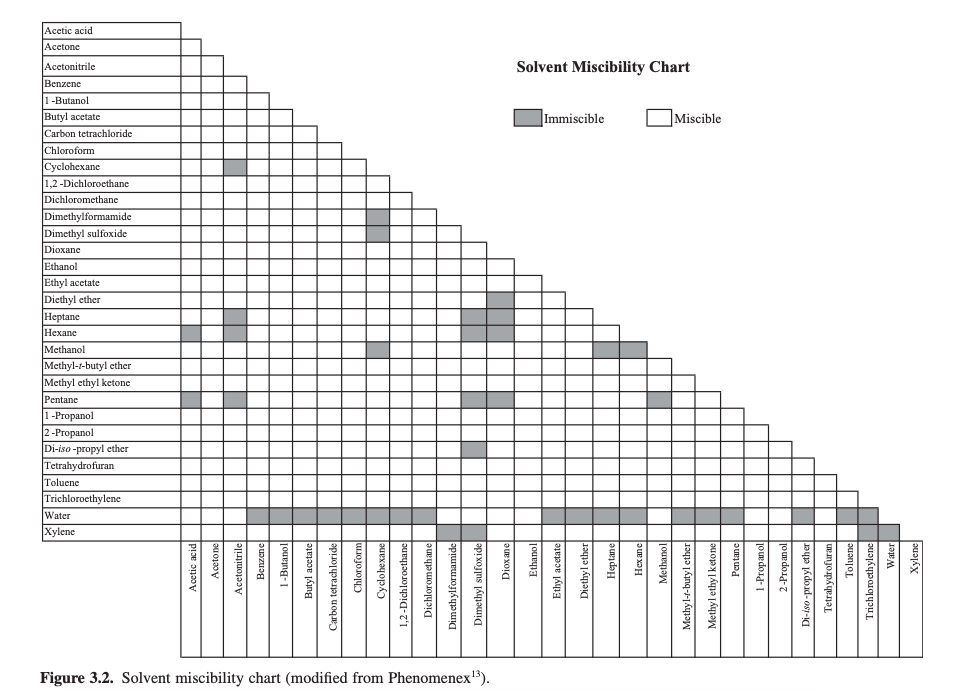
\includegraphics{../graphics/Solvent miscibility chart.png}\{\#fig:Solvent
miscibility chart\}

Trong nghiên cứu các hợp chất tự nhiên để tạo cao chiết thử tác dụng
sinh học để định hướng nhóm tác dụng trong thực vật, từ đó, phân lập và
xác định cấu trúc hóa học của hoạt chất có tác dụng sinh học, quy trình
mô tả dưới đây thường được áp dụng. Cao chiết từ thực vật sẽ được cô đặc
để loại bỏ dung môi chiết. Cao này sẽ được tái phân tán vào trong nước
với tỷ lệ thích hợp. Sau đó lắc phân đoạn lần lượt với các dung môi hữu
cơ có độ phân cực tăng dần gồm \emph{n}-hexan, Chloroform (khuyến cáo
thay thế bằng Dichloromethanol), Ethyl acetat và \emph{n}-butanol. Do
các dung môi này không đồng tan với nước dẫn đến để một thời gian sau sẽ
phân lớp. Các lớp dung mỗi giống nhau sẽ được gộp lại, loai bỏ dung môi
để thu được cao chiết. Kết quả là nhóm chất không phân cực như chất béo,
tinh dầu có xu hướng vào lớp dung môi \emph{n}-hexane, terpenoid và
alakaloid dạng base xu xướng vào lớp Chloroform (Dichloromethanol),
flavonoid xu hướng vào lớp Ethyl acetat trong khi saponin phân tốt trong
\emph{n}-butanol. Tuy nhiên, hợp chất tự nhiên đa dạng và trong hỗn hợp
có xu hướng tương tác với nhau dẫn tới quy trình này chỉ định hướng chứ
không đúng một cách tuyệt đối. \textbf{Giới hạn của phương pháp} Kỹ
thuật này cũng có một số nhược điểm ví dụ như quá trình vận hành thủ
công, tốn công sức và thời gian do cần thời gian để phân lớp giữa lớp
dung môi hữu cơ và lớp nước. Thêm nữa, các dung môi trên có thể gây vấn
đề về sức khỏe với người vận hành, tốn kém và gây ô nhiễm môi trường. Đề
khắc phục một số kỹ thuật đã được đề xuất như tối ưu hóa quy trình để
giảm mức sử dụng dung môi, giảm tiếp xúc với người lao
động.\textsuperscript{44,45}

** Thiết bị cải tiến chiết lỏng-lỏng hồi lưu liên tục (Continuous
liquid-liquid extraction) **

Thiết bị cải tiến chiết lỏng-lỏng hồi lưu liên tục là sự kết hợp giữa
quá trình chiết và bay hơi. Thiết bị đã thành công trong quá trình phân
tích thực phẩm, dược phẩm và các mẫu lâm sàng nhưng giảm thiểu ô
nhiễm.\textsuperscript{45} Mẫu được phân tán vào trong nước đặt tại bộ
phận chiết trong khi pha dung mỗi hưu cơ được nạp vào bộ phận có gia
nhiệt. Tùy thuộc vào tỷ trọng giữa pha phân tán và pha dung môi hữu cơ
mà chọn thiết bị như hình
\hyperref[fig:Extractionux5cux2520Apparatusux5cux2520Ofux5cux2520Thomas]{1.6}.
Pha dung môi hữu cơ hay pha chiết được gia nhiệt, dung môi sẽ bay hơi từ
bộ phận gia nhiệt bốc hơi và ngưng tự tại pha chiết theo từng giọt. Xuất
hiện sự trao đổi hoạt chất giữa pha nước và pha hữu cơ xảy ra mà không
cần khuấy trộn hay lắc để tăng sự tiếp xúc giữa hai pha dung môi không
đồng tan. Pha hữu cơ sẽ phân lớp và sẽ hồi lưu lại bộ phận có gia nhiệt.
Quá trình lặp đi lặp lại cho đến khi chiết phân đoạn kết thúc, nhóm chất
cần phân tích sẽ tách ra khỏi mẫu nền và thu lại tại bình gia nhiệt.
Thiết bị này cũng có khả năng giám sát chất lượng mẫu theo thời gian
thực khi bắt cặp với hệ thống MS, theo thiết kế của Hui-Hsien Yang và
cộng sự.\textsuperscript{46}

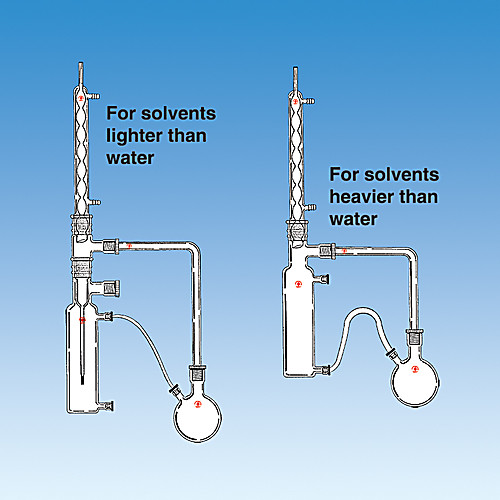
\includegraphics{../graphics/Extraction Apparatus Of Thomas.jpg}\{\#fig:Extraction
Apparatus Of Thomas\}

\subsection{1.6 Ứng dụng cao chiết trong ngành
dược}\label{ux1ee9ng-dux1ee5ng-cao-chiux1ebft-trong-nguxe0nh-dux1b0ux1ee3c}

\subsubsection{1.6.1 Cao chiết từ
lá}\label{cao-chiux1ebft-tux1eeb-luxe1}

Cao chiết từ lá đã được sử dụng để phòng và điều trị bệnh từ lâu. Ví dụ,
cao chiết từ lá của loài \emph{Olea europaea} (cây ô liu) để điều trị
cảm lạnh và cúm đã được sử dụng trong y học phương Tây. Ngày nay,
oleuropein, một seco-iridoid có khả năng kháng khuẩn, kháng viêm và
chống oxy hóa đã tìm thấy trong cao chiết từ lá ô liu. Bảng dưới liệt kê
một số trường hợp tác dụng sinh học của một số hoạt chất nằm trong cao
chiết từ lá một số dược liệu cũng như cách chiết xuất. Cao chiết từ
\emph{Olea europaea} (cây ô liu) cũng chứa một số hoạt chất khác có tác
dụng ức chế phát triển của virus và vi khuẩn. Chúng cũng xuất hiện trong
lá. Viêm họng sử dụng cao chiết từ lá để súc miệng có thể giảm triệu
chứng. Sử dụng cao chiết từ lá ô liu trong thời gian ngắn thường được
cho là an toàn nhưng thời gian dài chưa được chứng minh đầy đủ. Bệnh
nhân giai đoạn sớm của viêm khớp dạng thấp chiết xuất từ lá khô của ô
liu cùng methotrexate trong 6 tuần thấy giảm tổn thương tế bào, khôi
phục cân bằng chất chống oxy hóa, cải thiện khả năng ức chế IL-6. Tuy
nhiên với bệnh nhân mắc viêm khớp lâu năm thấy không có tác
dụng.\textsuperscript{47} Cao chiết bằng dung môi Ethanol của lá ô liu
xuất hiện một số nhóm nhất như phenolic, pentacyclic và alditols
triterpenes, tất cả đều có hoạt tính sinh học. Triterpene chính được tìm
thấy trong lá ô liu là acid oleanolic (3,0\% - 3,5\% DW), tiếp theo là
acid maslinic và một lượng nhỏ erythrodiol, caid ursolic và
uvaol.\textsuperscript{48}\\
Trong nhưng thập niêm gần đây, các polyphenol trong lá của loài
\emph{Camellia sinensis} (trà xanh) thu hút được quan tâm của nhiều nhà
nghiên cứu. Cao chiết trà xanh có hàm lượng cao của polyphenol,
flavonoid, caffein, acid amin, acid phenolic (đặc biệt là acid
hydroxybenzoic), carbohydrate, lipid và các hóa chất dễ bay hơi. Nhóm
Catechin, chẳng hạn như (-)-catechin (C), (-)-epigallocatechin gallate
(EGCG), (-)-epicatechin gallate (ECG), (-)-epicatechin (EC),
(-)-epigallocatechin (EGC) , (-)-gallocatechin gallate (GCG), và
(-)-gallocatechin (GC), là những thành phần polyphenol quan trọng
nhất.\textsuperscript{49} Dựa trên quá trình chế biến, ngoài trà xanh
còn có trà đen và trà ô long. Trà đen thu được từ quá trình lên men của
lá trà xanh và các catechin được chuyển đổi tạo ra màu sắc đen hơn cho
sản phẩm. Quá trình này làm giảm đáng kể nồng độ catechin trong trà đen.
Catechin, chẳng hạn như epigallocatechin và epigallocatechin gallate, có
nhiều trong trà xanh.\textsuperscript{50}\\
Thành phần hóa học và tác dụng sinh học của nhụy, vòi hoa, đài hoa, áo
hoa và lá của cây \emph{Crocus sativus} (Cây nghệ tây) đã được xác định
bởi Lahmass \emph{et al.} Các đặc điểm sinh học của nhụy (gia vị nghệ
tây) có liên quan đến hàm lượng cao của crocins. Mặc dù, tổng hàm lượng
phenolic và flavonoid cao hơn nhưng hoạt tính chống oxy hóa của cao
chiết tự nhụy nghệ tây thấp hơn so với cao chiết từ lá và hoa. Hiện tại
có ba cách giải thích cho những phát hiện này. Thứ nhất, lá có hàm lượng
luteolin và dẫn xuất glycosyl cao bất thường. Thứ hai, lá có chứa
kaempferol và dẫn xuất glycosyl. Và thứ ba, lá có hàm lượng cao các dẫn
xuất glycosyl của spaths có chứa crocin và các dẫn xuất
malvidin.\textsuperscript{51}\\
Lá cây \emph{Beta vulgaris L.} (củ cải đường) thường bị bỏ đi tuy nhiên
cao chiết từ lá chứa nồng độ cao phenolics, betacyanin và betaxanthin
được chứng minh bởi Bengardino \emph{et al.}\textsuperscript{52}
Betacyanins và betaxanthins (betalins) chứa nhóm nitơ và tan tốt trong
nước có hoạt tính sinh học. Tương tự như vậy, lá \emph{Curcuma longa L.}
(cây nghệ) cũng bị loại bỏ nhưng các nghiên cứu thấy cao chiết tự lá
nghệ an toàn dù chứa ít nitrat nhưng không chứa cyanua. Nếu sây khô bằng
vi sóng làm khô lá nghệ giúp tăng cường khả năng chống oxy hóa. Còn
nhiều bằng chứng nữa tác dụng của cao chiết từ lá dược liệu có tiềm năng
ngăn ngừa và điều trị bệnh.\textsuperscript{53,54}

\subsubsection{1.6.2 Cao chiết từ hoa và
quả}\label{cao-chiux1ebft-tux1eeb-hoa-vuxe0-quux1ea3}

Dầu thu được từ hạt thực vật có nhiều ứng dụng trong đời sống hàng ngày
cũng như trong dược phẩm. Đây có thể là sản phẩm phụ khi sử dụng trái
cây hoặc thu được trực tiếp. Hạt chứa hàm lượng cao các hoạt chất có
hoạt tính sinh học nếu so với các bộ phận khác từ quả và thường bị bỏ đi
trong nông nghiệp. Nếu sử dụng hạt để chiết xuất sẽ giảm thiểu đáng kể
các vấn đề rác thải nông nghiệp.\textsuperscript{55} Bước tiền xử lý hạt
cũng khá quan trọng. Hạt thu về phải được rửa sạch, loại bỏ vỏ hạt,
nghiền và sấy. Lớp màng xơ của hạt cũng cần loại bỏ vì chúng sẽ hút ẩm,
lên men làm hỏng hạt. Nghiền hạt đảm bảo phá vỡ và giải phóng dầu. Bên
cạnh đó, diện tích bề mặt tăng lên giúp dung môi tiếp xúc nhiều hơn với
tế bào và cho phép nâng cao hiệu suất chiết. Tiền xử lý bằng vi sóng đã
được chứng minh giúp cải tiện hiệu suất chiết dầu, nâng cao hàm lượng
tocopherols và phytosterols. Tuy nhiên, do quá trình phân hủy, tiền xử
lý hạt bằng vi sóng có thể làm giảm nồng độ acid béo không bão hòa
đa.\textsuperscript{56}\\
Các ví dụ khác nhau về việc phân lập các hoạt chất từ dịch chiết của hạt
thực vật được liệt kê trong Bảng dưới đây. Dầu thực vật từ lâu được xem
là nguồn cung cấp các vitamin tan trong dầu và các acid béo thiết yếu,
cũng như các thành phần hoạt tính sinh học khác bao gồm cả các hợp chất
dễ bay hơi. Cao chiết từ hạt thường có hoạt tính chống oxy hóa, kháng
khuẩn, kháng viêm, ứng chế tế bào ung thư, kháng virus và hạ đường
huyết. Hạ đường huyết của cao chiết từ hạt giúp kiểm soát đường huyết
bằng cách ức chế enzyem chuyển hóa carbohydrate. Nồng độ glucose máu
tăng sau bữa ăn do các enzyme thủy phân như amylase hay glucosidase. Các
phân tử tinh bột với khối lượng phân tử lớn không thể vượt qua màng ruột
sẽ được thủy phân thành phân tử có khối lượng nhỏ hơn dựa trên các
enzyme trên. Lượng đường trong máu sẽ tăng lên phụ thuộc vào tốc độ
chuyển hóa. Nếu lượng đường dư thừa sẽ được cơ thể chuyển hóa lưu trữ
trong tế bào dưới dạng glycogen nhờ các insulin. Nhờ khả năng ức chế
enzyme glucosidase (98,4\%) của cao chiết từ hạt \emph{Swietenia
macrophylla} (nhạc ngựa hay dái ngựa lá to, dái ngựa lá lớn, dái ngựa
Brasil, dái ngựa Honduras) có tác dụng như một thuốc điều trị đường
huyết. Tuy nhiên, tác dụng ức chế vừa phải hoạt động của enzyme amylase
(34,9\%). Khả năng ức chế virus của thảo mộc đóng vai trò quan trọng
trong điều trị virus. Để thay thế các thuốc hóa dược, một số công ty có
xu hướng sản xuất thuốc ức chế virus từ thảo mộc. Hoạt chất limonoid thu
được từ hạt cây \emph{Swietenia macrophylla} có tác dụng ức chế virus
gây sốt xuất huyết, lây truyền rộng rãi ở châu Á. Cao chiết từ hạt nho
chứa nhiều nhiều proanthocyanin đã được chứng minh có khả năng chống lại
virus viêm gan A và virus Tulane khi kết hợp với xử lý
nhiệt.\textsuperscript{57}\\
Một hoạt tính cần quan tâm cao chiết từ hạt là khả năng ức chế tế bào
ung thư. Theo nghiên cứu, khoảng 70\% polyphenol được tìm thấy với hàm
lượng cao trong hạt nho có đặc tính gây độc tế bào. Khả năng ức chế sự
phát triển tế bào ung thư biểu mô theo nồng độ và thời gian của hạt nho
hiệu quả hơn cao chiết từ vỏ nhỏ.\textsuperscript{58} Cao chiết tự hạt
bơ có khả năng ức chế tế bào ung thư thông qua chung trình chết tế bào
đã được chứng minh khi gây rối loạn chức năng tỷ thể với biểu hiện giải
phóng ra các phosphatidylserine. Cao chiết từ Vỏ hạt cây \emph{Paeonia
obovata} (thảo thược dược) có khả năng kháng khuẩn Gram dương bao gồm
\emph{Staphylococcus aureus}.\textsuperscript{59}\\
Thành phần có hoạt tính trong hoa cũng được phân lập và xác định cấu
trúc hóa học giống như trong hạt. Trigonelline, acid galic, caffein,
acid protocatechuic, cũng như melanoidin thuộc nhóm phenolic của hoa cà
phê. Nguyên \emph{et all} đã sử dụng kỹ thuật xanh để sản xuất cao có
hoạt tính sinh học với hàm lượng phenolic cao, melanoidin từ hoa cà
phê.\textsuperscript{60} Acid caffeic là thành phần acid hydroxycinnamic
dồi dào nhất trong cao chiết này tiếp theo là acid chlorogen, acid
ferulic và p-coumaric.

\subsubsection{1.6.3 Cao chiết từ vỏ
thân}\label{cao-chiux1ebft-tux1eeb-vux1ecf-thuxe2n}

Tương tự như lá cây, vỏ thân cây cũng chứa một số hoạt chất giống như
vậy. Bảng mô tả các ví dụ về chiết xuất cao chiết có hoạt tính từ vỏ
thân cây. Theo y học cổ truyền, vỏ thân của nhiều loài thực vật được sử
dụng để phòng và chữa bệnh. Ví dụ, vỏ cây thuộc chi Salix (chi liễu) đã
được sử dụng để điều trị sốt, khó chịu và viêm trong hàng ngàn năm.
Salicin, một hoạt chất có cấu trúc hóa học gần tương tự aspirin giúp
giảm đau và viêm được tìm thấy trong vỏ cây thuộc chi này. Vỏ cây thuộc
loài \emph{Rhamnus purshiana} (cây hắc mai, cây hắc mai California) được
sử dụng để điều trị táo bón và bệnh trĩ và trong một số liệu pháp điều
trị hậu phẫu trực tràng trong quá khứ. Trong vỏ cây xuất hiện một số dẫn
suất anthranoid có tác dụng nhuận tràng có cấu trúc hóa học ở dạng
anthraquinone tự do, dianthrones, anthrones và/hoặc O- và
C-glycoside.\textsuperscript{61} Trong những thập kỷ gần đây, nhiều nhà
nghiên cứu đã tiến hành phân lập các hợp chất có hoạt tính sinh học từ
thân cây. Ví dụ, scoparone, \(\beta\)-sitosterol, fraxidin, fraxetin,
acid 3-acetylaleuritolic và sitosterone từ vỏ thân cây \emph{Jatropha
podagrica} (Dầu lai có củ hay còn gọi dầu lai lá sen, sen lục
bình).\textsuperscript{62} Thengyai \emph{et al.} đã xác định vỏ thân là
bộ phận chứa hoạt tính sinh học cao nhất của của \emph{Vitex glabrata}
(cây mã).\textsuperscript{63} Tương tự, Minh \emph{et al.} đã xác định
và phân lập cấu trúc hóa học của acid galic, metyl gallat, fraxetin và
tomentin từ \emph{Jatropha podagrica}.\textsuperscript{62}

\subsubsection{1.6.4 Cao chiết từ rễ và thân
rễ}\label{cao-chiux1ebft-tux1eeb-rux1ec5-vuxe0-thuxe2n-rux1ec5}

Cao chiết từ rễ và thân rễ được sử dụng rộng khắp trên thế giới để điều
trị bệnh, phổ biến bao gồm gừng (\emph{Zingiber officinale}), maca
(\emph{Lepidium meyenii}), kava kava (\emph{Piper methysticum}), nghệ
(\emph{Curcuma longa}), cây nữ lang (\emph{Valeriana officinalis}), cúc
dại (\emph{Echinacea purpurea}), hải cẩu vàng (\emph{Hydrastis
canadensis}), sâm Ashwagandha (\emph{Withania somnifera}), và cam thảo
bắc (\emph{Glycyrrhiza glabra}). Gừng thường được sử làm gia vị tuy
nhiên cao chiết từ gừng có thể bào chế dưới dạng dung dịch đường uống,
viên nang cứng hoặc bột khô. Gừng được sử dụng để điều trị và ngăn ngừa
chứng buồn nôn do nhiều nguyên nhân bao gồm say tàu xe, ốm nghén và các
bệnh khác. Cao chiết từ gừng được chứng minh có khả năng chống viêm và
sử dụng trong điều trị các bệnh viêm khớp dạng thấp, viêm xương khớp,
đau cơ xương khớp. Một số thành phần có tác dụng đã được phân lập và xác
định cấu trúc với tác dụng tương tự như cao chiết gồm các hợp chất thuộc
nhóm gingerol và shogaol. Cao chiết từ gừng được chứng minh có khả năng
ức chế trực tiếp quá trình tổng hợp các chemokine từ hoạt dịch tế bào,
tế bào sụn và bạch cầu, rất có thể là do giảm sản xuất TNF và PGE-2
thông qua ức chế sự kích hoạt NFeB và IBalpha.\textsuperscript{64} Trong
của nghệ có chứa các hợp chất thuốc nhóm phenolic quan trọng là các
curcuminoid (2\% -9\%) gồm curcumin (70\%-75\%), demethoxycurcumin
(10\%-25\%) và bisdemethox-ycurcumin (5\% -10\% ).\textsuperscript{65}

\subsubsection{1.6.5 Cao chiết từ các bộ phận
khác}\label{cao-chiux1ebft-tux1eeb-cuxe1c-bux1ed9-phux1eadn-khuxe1c}

Lớp vỏ quả cà phê thường được bỏ đi cho thấy có tiềm năng sinh học khi
thử nghiệm \emph{in vitro} có khả năng chống oxy hóa và hàm lượng cao
các phenolics. Khi phân lập và xác định cấu trúc cho thấy cao chiết chứa
acid chlorogen (chủ yếu là acid 5-O-caffeoylquinic), acid caffeic và
caffein. Các hoạt chất này đều có tác dụng sinh học.\textsuperscript{66}
Trong các mô hình oxy hóa \emph{in vitro} và \emph{in vivo} (\emph{C.
elegans} được xử lý bằng tia cực tím), Iriondo-DeHond \emph{et al.} đã
phát hiện thấy cao chiết từ vỏ hạt có khả năng bảo vệ làn da và giảm
nguy cơ lão hóa trên da.\textsuperscript{67} Có vài đề xuất về khả năng
kháng viêm, các rối loạn mô mỡ nhờ vỏ quả cà phê.\textsuperscript{68}
Acid chlorogenic và kaempferol cũng tìm thấy trong cao chiết từ vỏ quả
cà phê.\\
Lớp vỏ mỏng của cà chua giàu lycopene có tác dụng tốt tới sức khỏe. Bã
quả cà chua là hỗn hợp vỏ và hạt sau khi chế biến cà chua đóng hộp trong
công nghiệp thực phần. Bã này chứa nhiều các carotenoid chủ yếu là
lycopene, lutein và caroten. Bã này cũng bao gồm các dẫn xuất acid béo
quan trọng mà cơ thể chúng ta cần.\textsuperscript{69}\\
Hành tây là cây gia vị phổ biến thứ hai trên thế giới và lớp vỏ cứng màu
vàng bị loại bỏ đi nhiều nhất. Đây là kết quả của quá trình sản xuất
công nghiệp thực phẩm. Trong lớp vỏ khô bỏ đi, thành phần flavonoid đặc
biệt giàu quercetin, các dẫn chất cũng như kaempferol và acid
protocatechuic. Sử dụng chiết xuất carbon dioxide và nước dưới tới hạn
sẽ thu được hiệu suất cao hơn hai lớp chất flavonoid và
phenolic.\textsuperscript{70,71}. Tương tự như vậy, actisô là nguồn cung
cấp các hoạt chất như các phenolic, inulin, cyclitols và sesquiterpenes.
Hơn nữa, có một lượng nhỏ hoạt chất có hoạt tính sinh học trong tất cả
các loại trái cây và rau quả chúng ta tiêu thụ hàng ngày. \#
Bibliography \{-\}

\phantomsection\label{refs}
\begin{CSLReferences}{0}{0}
\bibitem[\citeproctext]{ref-vinatoruOverviewUltrasonicallyAssisted2001}
\CSLLeftMargin{1 }%
\CSLRightInline{\href{https://doi.org/10.1016/S1350-4177(01)00071-2}{M.
Vinatoru, \emph{Ultrasonics Sonochemistry}, 2001, \textbf{8},
303--313}.}

\bibitem[\citeproctext]{ref-fitzgeraldMedicinalPlantAnalysis2020}
\CSLLeftMargin{2 }%
\CSLRightInline{\href{https://doi.org/10.3389/fphar.2019.01480}{M.
Fitzgerald, M. Heinrich and A. Booker, \emph{Front. Pharmacol.}, 2020,
\textbf{10}, 1480}.}

\bibitem[\citeproctext]{ref-rasulsuleriaBioactiveCompoundsPlant2019}
\CSLLeftMargin{3 }%
\CSLRightInline{H. A. Rasul Suleria and C. Barrow, \emph{Bioactive
{Compounds} from {Plant Origins}: {Extraction}, {Applications}, and
{Potential Health Benefits}}, {Apple Academic Press, Incorporated},
{Milton}, 2019.}

\bibitem[\citeproctext]{ref-limaPolyphenolsFruitsVegetables2014}
\CSLLeftMargin{4 }%
\CSLRightInline{\href{https://doi.org/10.4236/fns.2014.511117}{G. P. P.
Lima, F. Vianello, C. R. Corrêa, R. A. da S. Campos and M. G. Borguini,
\emph{FNS}, 2014, \textbf{05}, 1065--1082}.}

\bibitem[\citeproctext]{ref-kris-ethertonBioactiveCompoundsNutrition2004}
\CSLLeftMargin{5 }%
\CSLRightInline{\href{https://doi.org/10.1146/annurev.nutr.23.011702.073237}{P.
M. Kris-Etherton, M. Lefevre, G. R. Beecher, M. D. Gross, C. L. Keen and
T. D. Etherton, \emph{Annu. Rev. Nutr.}, 2004, \textbf{24}, 511--538}.}

\bibitem[\citeproctext]{ref-levyChangesIntestinalFlora1976}
\CSLLeftMargin{6 }%
\CSLRightInline{\href{https://doi.org/10.1056/NEJM197609092951103}{S. B.
Levy, G. B. FitzGerald and A. B. Macone, \emph{N Engl J Med}, 1976,
\textbf{295}, 583--588}.}

\bibitem[\citeproctext]{ref-fordFruitVegetableConsumption2001}
\CSLLeftMargin{7 }%
\CSLRightInline{\href{https://doi.org/10.1006/pmed.2000.0772}{E. S. Ford
and A. H. Mokdad, \emph{Preventive Medicine}, 2001, \textbf{32},
33--39}.}

\bibitem[\citeproctext]{ref-jCommentaryResveratrol2015}
\CSLLeftMargin{8 }%
\CSLRightInline{C. J, \emph{Med Aromat Plants},
DOI:\href{https://doi.org/10.4172/2167-0412.1000206}{10.4172/2167-0412.1000206}.}

\bibitem[\citeproctext]{ref-ferrieresFrenchParadoxLessons2004}
\CSLLeftMargin{9 }%
\CSLRightInline{\href{https://doi.org/10.1136/heart.90.1.107}{J.
Ferrieres, \emph{Heart}, 2004, \textbf{90}, 107--111}.}

\bibitem[\citeproctext]{ref-croteauTaxolBiosynthesisMolecular2006}
\CSLLeftMargin{10 }%
\CSLRightInline{\href{https://doi.org/10.1007/s11101-005-3748-2}{R.
Croteau, R. E. B. Ketchum, R. M. Long, R. Kaspera and M. R. Wildung,
\emph{Phytochem Rev}, 2006, \textbf{5}, 75--97}.}

\bibitem[\citeproctext]{ref-taiz2015plant}
\CSLLeftMargin{11 }%
\CSLRightInline{L. Taiz, E. Zeiger, I. M. Møller, A. Murphy and others,
\emph{Plant physiology and development.}, {Sinauer Associates
Incorporated}, 2015.}

\bibitem[\citeproctext]{ref-singhPlantTerpenesDefense2015}
\CSLLeftMargin{12 }%
\CSLRightInline{\href{https://doi.org/10.1007/s13205-014-0220-2}{B.
Singh and R. A. Sharma, \emph{3 Biotech}, 2015, \textbf{5}, 129--151}.}

\bibitem[\citeproctext]{ref-langeMetabolicEngineeringPlant2013}
\CSLLeftMargin{13 }%
\CSLRightInline{\href{https://doi.org/10.1111/pbi.12022}{B. M. Lange and
A. Ahkami, \emph{Plant Biotechnol J}, 2013, \textbf{11}, 169--196}.}

\bibitem[\citeproctext]{ref-callistoLeafLitterPossible2007}
\CSLLeftMargin{14 }%
\CSLRightInline{\href{https://doi.org/10.1590/S0101-81752007000200023}{M.
Callisto, J. F. Gonçalves Jr and M. A. S. Graça, \emph{Rev. Bras.
Zool.}, 2007, \textbf{24}, 442--448}.}

\bibitem[\citeproctext]{ref-phamkimBaoCaoTong1996}
\CSLLeftMargin{15 }%
\CSLRightInline{M. Phạm Kim, \emph{Báo cáo tổng kết nghiên cứu công nghệ
chiết xuất Diosgenin làm nghiên liệu chế tạo các thuốc Steroit}, {Viện
Dược liệu}, {Hà nội}, 1996.}

\bibitem[\citeproctext]{ref-vranovaStructureDynamicsIsoprenoid2012}
\CSLLeftMargin{16 }%
\CSLRightInline{\href{https://doi.org/10.1093/mp/sss015}{E. Vranová, D.
Coman and W. Gruissem, \emph{Molecular Plant}, 2012, \textbf{5},
318--333}.}

\bibitem[\citeproctext]{ref-heinrichAlkaloidsUsedMedicines2021}
\CSLLeftMargin{17 }%
\CSLRightInline{\href{https://doi.org/10.3390/molecules26071836}{M.
Heinrich, J. Mah and V. Amirkia, \emph{Molecules}, 2021, \textbf{26},
1836}.}

\bibitem[\citeproctext]{ref-kolakEffectsChronicRosiglitazone2007}
\CSLLeftMargin{18 }%
\CSLRightInline{\href{https://doi.org/2016092613233300554}{M. Kolak, H.
Yki-Järvinen, K. Kannisto, M. Tiikkainen, A. Hamsten, P. Eriksson and R.
M. Fisher, \emph{The Journal of Clinical Endocrinology \& Metabolism},
2007, \textbf{92}, 720--724}.}

\bibitem[\citeproctext]{ref-aniszewski2015alkaloids}
\CSLLeftMargin{19 }%
\CSLRightInline{T. Aniszewski,
\emph{\href{https://books.google.com.vn/books?id=tQ6dBAAAQBAJ}{Alkaloids:
{Chemistry}, biology, ecology, and applications}}, {Elsevier Science},
2015.}

\bibitem[\citeproctext]{ref-williamsonBioavailabilityBioefficacyPolyphenols2005}
\CSLLeftMargin{20 }%
\CSLRightInline{\href{https://doi.org/10.1093/ajcn/81.1.243S}{G.
Williamson and C. Manach, \emph{The American Journal of Clinical
Nutrition}, 2005, \textbf{81}, 243S--255S}.}

\bibitem[\citeproctext]{ref-govindarajanTurmericChemistryTechnology1980}
\CSLLeftMargin{21 }%
\CSLRightInline{\href{https://doi.org/10.1080/10408398009527278}{V. S.
Govindarajan and W. H. Stahl, \emph{C R C Critical Reviews in Food
Science and Nutrition}, 1980, \textbf{12}, 199--301}.}

\bibitem[\citeproctext]{ref-linDeterminationPterostilbeneRat2009}
\CSLLeftMargin{22 }%
\CSLRightInline{\href{https://doi.org/10.1002/bmc.1254}{H.-S. Lin, B.-D.
Yue and P. C. Ho, \emph{Biomed. Chromatogr.}, 2009, \textbf{23},
1308--1315}.}

\bibitem[\citeproctext]{ref-kahkonenAntioxidantActivityPlant1999}
\CSLLeftMargin{23 }%
\CSLRightInline{\href{https://doi.org/10.1021/jf990146l}{M. P. Kähkönen,
A. I. Hopia, H. J. Vuorela, J.-P. Rauha, K. Pihlaja, T. S. Kujala and M.
Heinonen, \emph{J. Agric. Food Chem.}, 1999, \textbf{47}, 3954--3962}.}

\bibitem[\citeproctext]{ref-cheynierPolyphenolsFoodsAre2005}
\CSLLeftMargin{24 }%
\CSLRightInline{\href{https://doi.org/10.1093/ajcn/81.1.223S}{V.
Cheynier, \emph{The American Journal of Clinical Nutrition}, 2005,
\textbf{81}, 223S--229S}.}

\bibitem[\citeproctext]{ref-croftChemistryBiologicalEffects1998}
\CSLLeftMargin{25 }%
\CSLRightInline{\href{https://doi.org/10.1111/j.1749-6632.1998.tb09922.x}{K.
D. Croft, \emph{Annals NY Acad Sci}, 1998, \textbf{854}, 435--442}.}

\bibitem[\citeproctext]{ref-puriPhytochemicalDictionary1998}
\CSLLeftMargin{26 }%
\CSLRightInline{B. Puri and A. Hall,
\emph{\href{https://doi.org/10.4324/9780203483756}{Phytochemical
{Dictionary}}}, {CRC Press}, 0th edn., 1998.}

\bibitem[\citeproctext]{ref-ganiWholeGrainCerealBioactive00}
\CSLLeftMargin{27 }%
\CSLRightInline{\href{https://doi.org/10.4172/2157-7110.1000146}{A.
Gani, W. Sm, M. Fa and G. Hameed, \emph{Journal of Food Processing \&
Technology}, \textbf{3}, 1--10}.}

\bibitem[\citeproctext]{ref-mollerBioactivePeptidesProteins2008}
\CSLLeftMargin{28 }%
\CSLRightInline{\href{https://doi.org/10.1007/s00394-008-0710-2}{N. P.
Möller, K. E. Scholz-Ahrens, N. Roos and J. Schrezenmeir, \emph{Eur J
Nutr}, 2008, \textbf{47}, 171--182}.}

\bibitem[\citeproctext]{ref-kittsBioactiveProteinsPeptides2003}
\CSLLeftMargin{29 }%
\CSLRightInline{\href{https://doi.org/10.2174/1381612033454883}{D. Kitts
and K. Weiler, \emph{CPD}, 2003, \textbf{9}, 1309--1323}.}

\bibitem[\citeproctext]{ref-xiaoDietaryFlavonoidAglycones2015}
\CSLLeftMargin{30 }%
\CSLRightInline{\href{https://doi.org/10.1080/10408398.2015.1032400}{J.
Xiao, \emph{Critical Reviews in Food Science and Nutrition}, 2015,
00--00}.}

\bibitem[\citeproctext]{ref-ohtaniSelectiveCleavageEster1984}
\CSLLeftMargin{31 }%
\CSLRightInline{\href{https://doi.org/10.1016/S0040-4039(01)81487-8}{K.
Ohtani, K. Mizutani, R. Kasai and O. Tanaka, \emph{Tetrahedron Letters},
1984, \textbf{25}, 4537--4540}.}

\bibitem[\citeproctext]{ref-joanagil-chavezTechnologiesExtractionProduction2013}
\CSLLeftMargin{32 }%
\CSLRightInline{\href{https://doi.org/10.1111/1541-4337.12005}{G. Joana
Gil-Chávez, J. A. Villa, J. Fernando Ayala-Zavala, J. Basilio Heredia,
D. Sepulveda, E. M. Yahia and G. A. González-Aguilar, \emph{Compr. Rev.
Food Sci. Food Saf.}, 2013, \textbf{12}, 5--23}.}

\bibitem[\citeproctext]{ref-azmirTechniquesExtractionBioactive2013}
\CSLLeftMargin{33 }%
\CSLRightInline{\href{https://doi.org/10.1016/j.jfoodeng.2013.01.014}{J.
Azmir, I. S. M. Zaidul, M. M. Rahman, K. M. Sharif, A. Mohamed, F.
Sahena, M. H. A. Jahurul, K. Ghafoor, N. A. N. Norulaini and A. K. M.
Omar, \emph{Journal of Food Engineering}, 2013, \textbf{117},
426--436}.}

\bibitem[\citeproctext]{ref-ajikumarTerpenoidsOpportunitiesBiosynthesis2008}
\CSLLeftMargin{34 }%
\CSLRightInline{\href{https://doi.org/10.1021/mp700151b}{P. K. Ajikumar,
K. Tyo, S. Carlsen, O. Mucha, T. H. Phon and G. Stephanopoulos,
\emph{Mol. Pharmaceutics}, 2008, \textbf{5}, 167--190}.}

\bibitem[\citeproctext]{ref-ingler.HeterocyclicChemistryBenzimidazoles2011}
\CSLLeftMargin{35 }%
\CSLRightInline{R. Ingle,.}

\bibitem[\citeproctext]{ref-delorsLearningTreasureReport1996}
\CSLLeftMargin{36 }%
\CSLRightInline{J. Delors,
\emph{\href{https://unesdoc.unesco.org/ark:/48223/pf0000109590}{Learning:
The treasure within; report to {UNESCO} of the {International
Commission} on {Education} for the {Twenty-first Century} (highlights) -
{UNESCO Digital Library}}}, 1996.}

\bibitem[\citeproctext]{ref-donsiApplicationsPulsedElectric2010}
\CSLLeftMargin{37 }%
\CSLRightInline{\href{https://doi.org/10.1007/s12393-010-9015-3}{F.
Donsì, G. Ferrari and G. Pataro, \emph{Food Eng. Rev.}, 2010,
\textbf{2}, 109--130}.}

\bibitem[\citeproctext]{ref-bernalAcuteLiverFailure2010}
\CSLLeftMargin{38 }%
\CSLRightInline{\href{https://doi.org/10.1016/S0140-6736(10)60274-7}{W.
Bernal, G. Auzinger, A. Dhawan and J. Wendon, \emph{The Lancet}, 2010,
\textbf{376}, 190--201}.}

\bibitem[\citeproctext]{ref-dayIncorporationFunctionalIngredients2009}
\CSLLeftMargin{39 }%
\CSLRightInline{\href{https://doi.org/10.1016/j.tifs.2008.05.002}{L.
Day, R. B. Seymour, K. F. Pitts, I. Konczak and L. Lundin, \emph{Trends
in Food Science \& Technology}, 2009, \textbf{20}, 388--395}.}

\bibitem[\citeproctext]{ref-plazaSearchNewFunctional2008}
\CSLLeftMargin{40 }%
\CSLRightInline{\href{https://doi.org/10.1016/j.tifs.2007.07.012}{M.
Plaza, A. Cifuentes and E. Ibanez, \emph{Trends in Food Science \&
Technology}, 2008, \textbf{19}, 31--39}.}

\bibitem[\citeproctext]{ref-maretteFunctionalFoodUncertainty2010}
\CSLLeftMargin{41 }%
\CSLRightInline{\href{https://doi.org/10.1016/j.foodpol.2010.04.009}{S.
Marette, J. Roosen, S. Blanchemanche and E. Feinblatt-Mélèze, \emph{Food
Policy}, 2010, \textbf{35}, 419--428}.}

\bibitem[\citeproctext]{ref-nobiliNaturalCompoundsCancer2009}
\CSLLeftMargin{42 }%
\CSLRightInline{\href{https://doi.org/10.1016/j.phrs.2009.01.017}{S.
Nobili, D. Lippi, E. Witort, M. Donnini, L. Bausi, E. Mini and S.
Capaccioli, \emph{Pharmacological Research}, 2009, \textbf{59},
365--378}.}

\bibitem[\citeproctext]{ref-hekmatGrowthSurvivalLactobacillus2009}
\CSLLeftMargin{43 }%
\CSLRightInline{\href{https://doi.org/10.1016/j.ifset.2008.10.007}{S.
Hekmat, H. Soltani and G. Reid, \emph{Innovative Food Science \&
Emerging Technologies}, 2009, \textbf{10}, 293--296}.}

\bibitem[\citeproctext]{ref-miroRecentDevelopmentsAutomatic2008}
\CSLLeftMargin{44 }%
\CSLRightInline{\href{https://doi.org/10.1016/j.trac.2008.07.003}{M.
Miró, S. K. Hartwell, J. Jakmunee, K. Grudpan and E. H. Hansen,
\emph{TrAC Trends in Analytical Chemistry}, 2008, \textbf{27},
749--761}.}

\bibitem[\citeproctext]{ref-hiiLiquidLiquidExtractionEnvironmental2011}
\CSLLeftMargin{45 }%
\CSLRightInline{\href{https://doi.org/10.1002/9780813823621.ch3}{T. M.
Hii and H. K. Lee, in \emph{Handbook of {Sample Preparation}}, eds. J.
Pawliszyn and H. L. Lord, {John Wiley \& Sons, Inc.}, {Hoboken, NJ,
USA}, 2011, pp. 39--51}.}

\bibitem[\citeproctext]{ref-yangKineticStudyContinuous2018}
\CSLLeftMargin{46 }%
\CSLRightInline{\href{https://doi.org/10.1016/j.aca.2018.06.072}{H.-H.
Yang, E. P. Dutkiewicz and P. L. Urban, \emph{Analytica Chimica Acta},
2018, \textbf{1034}, 85--91}.}

\bibitem[\citeproctext]{ref-oliveiraOliveLeafPhenolic2021}
\CSLLeftMargin{47 }%
\CSLRightInline{\href{https://doi.org/10.1016/j.jece.2021.106175}{A. L.
S. Oliveira, S. Gondim, R. Gómez-García, T. Ribeiro and M. Pintado,
\emph{Journal of Environmental Chemical Engineering}, 2021, \textbf{9},
106175}.}

\bibitem[\citeproctext]{ref-lama-munozContentPhenolicCompounds2020}
\CSLLeftMargin{48 }%
\CSLRightInline{\href{https://doi.org/10.1016/j.foodchem.2020.126626}{A.
Lama-Muñoz, M. del M. Contreras, F. Espínola, M. Moya, I. Romero and E.
Castro, \emph{Food Chemistry}, 2020, \textbf{320}, 126626}.}

\bibitem[\citeproctext]{ref-hsounaCharacterizationBioactiveCompounds2011}
\CSLLeftMargin{49 }%
\CSLRightInline{\href{https://doi.org/10.1016/j.fct.2011.09.034}{A. B.
Hsouna, M. Saoudi, M. Trigui, K. Jamoussi, T. Boudawara, S. Jaoua and A.
E. Feki, \emph{Food and Chemical Toxicology}, 2011, \textbf{49},
3183--3191}.}

\bibitem[\citeproctext]{ref-korystovaBlackTeaMore2021}
\CSLLeftMargin{50 }%
\CSLRightInline{\href{https://doi.org/10.1016/j.biopha.2021.112064}{A.
F. Korystova, L. N. Kublik, T. V. Samokhvalova, V. V. Shaposhnikova and
Y. N. Korystov, \emph{Biomedicine \& Pharmacotherapy}, 2021,
\textbf{142}, 112064}.}

\bibitem[\citeproctext]{ref-bragaCurcumaLongaLeaves2018}
\CSLLeftMargin{51 }%
\CSLRightInline{\href{https://doi.org/10.1016/j.foodchem.2018.05.096}{M.
C. Braga, E. C. S. Vieira and T. F. de Oliveira, \emph{Food Chemistry},
2018, \textbf{265}, 308--315}.}

\bibitem[\citeproctext]{ref-cabarkapaDryOliveLeaf2016}
\CSLLeftMargin{52 }%
\CSLRightInline{\href{https://doi.org/10.1002/ptr.5662}{A. Čabarkapa, L.
Živković, S. Borozan, M. Zlatković-Švenda, D. Dekanski, I. Jančić, M.
Radak-Perović, V. Bajić and B. Spremo-Potparević, \emph{Phytother.
Res.}, 2016, \textbf{30}, 1615--1623}.}

\bibitem[\citeproctext]{ref-haldarReviewEnvironmentfriendlyEmerging2021}
\CSLLeftMargin{53 }%
\CSLRightInline{\href{https://doi.org/10.1016/j.chemosphere.2020.128523}{D.
Haldar and M. K. Purkait, \emph{Chemosphere}, 2021, \textbf{264},
128523}.}

\bibitem[\citeproctext]{ref-haldarLignocellulosicConversionValueadded2020}
\CSLLeftMargin{54 }%
\CSLRightInline{\href{https://doi.org/10.1016/j.procbio.2019.10.001}{D.
Haldar and M. K. Purkait, \emph{Process Biochemistry}, 2020,
\textbf{89}, 110--133}.}

\bibitem[\citeproctext]{ref-gomez-mejiaValorisationBlackMulberry2021}
\CSLLeftMargin{55 }%
\CSLRightInline{\href{https://doi.org/10.1016/j.foodchem.2020.127998}{E.
Gómez-Mejía, C. L. Roriz, S. A. Heleno, R. Calhelha, M. I. Dias, J.
Pinela, N. Rosales-Conrado, M. E. León-González, I. C. F. R. Ferreira
and L. Barros, \emph{Food Chemistry}, 2021, \textbf{337}, 127998}.}

\bibitem[\citeproctext]{ref-fathi-achachloueiMicrowavePretreatmentPromising2019}
\CSLLeftMargin{56 }%
\CSLRightInline{\href{https://doi.org/10.1016/j.indcrop.2018.11.034}{B.
Fathi-Achachlouei, S. Azadmard-Damirchi, Y. Zahedi and R. Shaddel,
\emph{Industrial Crops and Products}, 2019, \textbf{128}, 527--533}.}

\bibitem[\citeproctext]{ref-patwardhanHeatSensitizationHepatitis2020}
\CSLLeftMargin{57 }%
\CSLRightInline{\href{https://doi.org/10.1016/j.fm.2020.103461}{M.
Patwardhan, M. T. Morgan, V. Dia and D. H. D'Souza, \emph{Food
Microbiology}, 2020, \textbf{90}, 103461}.}

\bibitem[\citeproctext]{ref-dimeoAnticancerActivityGrape2019}
\CSLLeftMargin{58 }%
\CSLRightInline{\href{https://doi.org/10.1016/j.jff.2019.103515}{F. Di
Meo, R. Aversano, G. Diretto, O. C. Demurtas, C. Villano, S. Cozzolino,
S. Filosa, D. Carputo and S. Crispi, \emph{Journal of Functional Foods},
2019, \textbf{61}, 103515}.}

\bibitem[\citeproctext]{ref-yanInsightsPhytochemicalComposition2020}
\CSLLeftMargin{59 }%
\CSLRightInline{\href{https://doi.org/10.3390/plants9060729}{Z. Yan, L.
Xie, Y. Tian, M. Li, J. Ni, Y. Zhang and L. Niu, \emph{Plants}, 2020,
\textbf{9}, 729}.}

\bibitem[\citeproctext]{ref-nguyenUseCoffeeFlower2019}
\CSLLeftMargin{60 }%
\CSLRightInline{\href{https://doi.org/10.1016/j.foodchem.2019.125120}{T.
M. T. Nguyen, E. J. Cho, Y. Song, C. H. Oh, R. Funada and H.-J. Bae,
\emph{Food Chemistry}, 2019, \textbf{299}, 125120}.}

\bibitem[\citeproctext]{ref-minhIsolationPurificationBioactive2019}
\CSLLeftMargin{61 }%
\CSLRightInline{\href{https://doi.org/10.3390/molecules24050889}{T.
Minh, T. Xuan, H.-D. Tran, T. Van, Y. Andriana, T. Khanh, N. Quan and A.
Ahmad, \emph{Molecules}, 2019, \textbf{24}, 889}.}

\bibitem[\citeproctext]{ref-nurjanahBioactiveCompoundsAntioxidant2015}
\CSLLeftMargin{62 }%
\CSLRightInline{N. Nurjanah, A. M. Jacoeb, T. Hidayat and A. Shylina,.}

\bibitem[\citeproctext]{ref-thengyaiAGlucosidaseAamylaseInhibitory2020}
\CSLLeftMargin{63 }%
\CSLRightInline{\href{https://doi.org/10.1016/j.hermed.2019.100302}{S.
Thengyai, P. Thiantongin, C. Sontimuang, C. Ovatlarnporn and P.
Puttarak, \emph{Journal of Herbal Medicine}, 2020, \textbf{19},
100302}.}

\bibitem[\citeproctext]{ref-deoliveirafilhoBioactiveCompoundsTurmeric2021}
\CSLLeftMargin{64 }%
\CSLRightInline{\href{https://doi.org/10.1007/978-3-030-57415-4_37}{J.
G. de Oliveira Filho, M. J. de Almeida, T. L. Sousa, D. C. dos Santos
and M. B. Egea, in \emph{Bioactive {Compounds} in {Underutilized
Vegetables} and {Legumes}}, eds. H. N. Murthy and K. Y. Paek, {Springer
International Publishing}, {Cham}, 2021, pp. 297--318}.}

\bibitem[\citeproctext]{ref-latviauniversityoflifesciencesandtechnologiesBioactiveCompoundsFresh2019}
\CSLLeftMargin{65 }%
\CSLRightInline{\href{https://doi.org/10.22616/FoodBalt.2019.050}{Latvia
University of Life Sciences and Technologies, B. Ozola, I. Augspole, M.
Duma and V. Kreicbergs, 2019, pp. 265--268}.}

\bibitem[\citeproctext]{ref-bessadaCoffeaCanephoraSilverskin2018}
\CSLLeftMargin{66 }%
\CSLRightInline{\href{https://doi.org/10.1016/j.scitotenv.2018.07.201}{S.
M. F. Bessada, R. C. Alves, A. S. G. Costa, M. A. Nunes and M. B. P. P.
Oliveira, \emph{Science of The Total Environment}, 2018, \textbf{645},
1021--1028}.}

\bibitem[\citeproctext]{ref-iriondo-dehondCoffeeSilverskinExtract2016}
\CSLLeftMargin{67 }%
\CSLRightInline{\href{https://doi.org/10.3390/molecules21060721}{A.
Iriondo-DeHond, P. Martorell, S. Genovés, D. Ramón, K. Stamatakis, M.
Fresno, A. Molina and M. del Castillo, \emph{Molecules}, 2016,
\textbf{21}, 721}.}

\bibitem[\citeproctext]{ref-rebollo-hernanzPhenolicCompoundsCoffee2019}
\CSLLeftMargin{68 }%
\CSLRightInline{\href{https://doi.org/10.1016/j.fct.2019.110672}{M.
Rebollo-Hernanz, Q. Zhang, Y. Aguilera, M. A. Martín-Cabrejas and E.
Gonzalez de Mejia, \emph{Food and Chemical Toxicology}, 2019,
\textbf{132}, 110672}.}

\bibitem[\citeproctext]{ref-szaboAntimicrobialAntioxidantProperties2019}
\CSLLeftMargin{69 }%
\CSLRightInline{\href{https://doi.org/10.1016/j.lwt.2019.108558}{K.
Szabo, F. V. Dulf, Z. Diaconeasa and D. C. Vodnar, \emph{LWT}, 2019,
\textbf{116}, 108558}.}

\bibitem[\citeproctext]{ref-munirSubcriticalWaterExtraction2018}
\CSLLeftMargin{70 }%
\CSLRightInline{\href{https://doi.org/10.1016/j.jclepro.2018.02.166}{M.
T. Munir, H. Kheirkhah, S. Baroutian, S. Y. Quek and B. R. Young,
\emph{Journal of Cleaner Production}, 2018, \textbf{183}, 487--494}.}

\bibitem[\citeproctext]{ref-camponeResponseSurfaceMethodology2018}
\CSLLeftMargin{71 }%
\CSLRightInline{\href{https://doi.org/10.1016/j.foodchem.2018.07.042}{L.
Campone, R. Celano, A. Lisa Piccinelli, I. Pagano, S. Carabetta, R. D.
Sanzo, M. Russo, E. Ibañez, A. Cifuentes and L. Rastrelli, \emph{Food
Chemistry}, 2018, \textbf{269}, 495--502}.}

\end{CSLReferences}




\end{document}
